% siminos/schur/DingCvit14.tex      dvips DingCvit14
% $Author: xiong $ $Date: 2016-05-11 11:47:21 -0400 (Wed, 11 May 2016) $

                        %% logical setup, no need to edit %%%%%%%%%%
                        \newif\ifboyscout                         %%
                        \boyscouttrue %% commented, WWW/boyscouts %%
                        \newif\ifhighlightedits                   %%
                        \highlighteditstrue                       %%
                        \newif\ifpreparepdf                       %%
                        \preparepdftrue % hyperlinked pdf default %%

                        % Toggle between draft and non-draft versions
% \boyscoutfalse                 % public, hyperlinked
% \preparepdffalse               % for B&W, print version

% Predrag       almost there         Jun 14 2014
% Xiong Ding    1. draft             Feb 18 2014


%% ------------------ for arXiv submission ----------------------------
%
% Title:    Periodic eigendecomposition and its application to
%           Kuramoto-Sivashinsky system
% Authors:  Xiong Ding and Predrag Cvitanovi\'c
% Comments: 18 pages, 3 postscript figures, uses siamltex1213.cls
% Category:
% Files:    DingCvit14.tex defsSchur.tex DingCvit14.bbl
%           pprpfigure.eps ppo1vectfield.eps  rpo1_marginal3.eps
%
%% ------------------ cut here ----------------------------------------


\documentclass[final,leqno,onefignum,onetabnum]{siamltexmm}

\input defsSchur

% SIAM Journal on Applied Dynamical Systems style
\usepackage{amsmath,amssymb}
\usepackage{amsfonts}
\usepackage{graphicx}
\usepackage{subfigure}
\usepackage{dsfont}
\usepackage{mathrsfs}
\bibliographystyle{hsiam}
% Xiong had \bibliographystyle{siam}

\usepackage{ifthen}
\usepackage{tikz}
\usetikzlibrary{calc}
\usetikzlibrary{decorations.pathreplacing}
%\usepackage{array}
\graphicspath{{./figs/}}

%\linespread{1.5} % set double line space.

\title{
Periodic eigendecomposition and its application to
Kuramoto-Sivashinsky system
}

\author{
  Xiong Ding\footnotemark[2]
  \and
  Predrag Cvitanovi\'{c}\footnotemark[2]
}

\begin{document}
\maketitle
\newcommand{\slugmaster}{%
\slugger{siads}{xxxx}{xx}{x}{x--x}}
%slugger should be set to mms, siap, sicomp, sicon, sidma, sima,
%                        simax, sinum, siopt, sisc, or sirev

\renewcommand{\thefootnote}{\fnsymbol{footnote}}
\footnotetext[2]{
Center for Nonlinear Science,
School of Physics,
Georgia Institute of Technology, Atlanta, GA 30332
(\href{mailto:xding@gatech.edu}{xding@gatech.edu},
\href{mailto:predrag.cvitanovic@physics.gatech.edu}{predrag.cvitanovic@physics.gatech.edu}).
} % footnote marker begins with 2 because the first one is reserved for
  % date-received information

\begin{abstract}
\Ped, to be formulated in this paper,
is a numerical method to compute Floquet spectrum and \Fv s along
periodic orbits in a dynamical system. It is rooted in
numerical algorithm advances in computation
of \edit{\cLvs}
of the linearized flow along an ergodic trajectory in a chaotic
system. Also, we incorporate \psd\ to the computation of
\Fv s, compare it with other
methods, and show that \ped\ can yield
\edit{the full set of Floquet vectors}
of a periodic orbit at every point along the orbit to high accuracy.
Its power, and in particular its ability to resolve eigenvalues
differing by hundreds of orders of magnitude, is demonstrated by
applying the algorithm to computation of the full linear stability
spectrum of several periodic solutions in one dimensional
Kuramoto-Sivashinsky flow.
\end{abstract}

\begin{keywords}
\ped, \psd, periodic Sylvester equation,
\edit{\cLvs}, Floquet
vectors, \KS, linear stability, continuous symmetry
\end{keywords}

\begin{AMS}
  15A18, 35B10, 37L20, 37M25, 65F15, 65H10, 65P20, 65P40, 76F20
\end{AMS}
\pagestyle{myheadings}
\thispagestyle{plain}
\markboth{XIONG~DING AND PREDRAG~CVITANOVI\'C}{PERIODIC EIGENDECOMPOSITION}

\section{Introduction}
\label{sect:intro}

In dissipative chaotic dynamical systems, the decomposition of the
tangent space of invariant subsets into
stable, unstable and center subspaces is important for analyzing the
geometrical structure of the solution field\rf{guckb}.
For equilibrium \edit{states},
the task is quite simple, which is reduced to the eigen-problem of
a single stability matrix, but the scenario is much more difficult
for complex structures, such as periodic orbits and invariant \edit{tori},
since the expansion/contraction rates in high dimensional systems usually
span a large range of \edit{orders of} magnitude. Actually, in literature, two different
algorithms are capable of resolving this problem partially originated
from different settings. The first candidate is \cLv\
algorithm\edit{\rf{GiChLiPo12, ginelli-2007-99, KuPa12, WoSa07}}.
It is designed to stratify the Oseledets subspaces\rf{lyaos, ruelle79}
corresponding to
the hierarchy of Lyapunov exponents along a long non-wandering orbit
on the attractor. \CLv s attract a lot of attention in the past few
years. They
turn out to be a useful tool for physicists
to investigate the dynamical properties of the system, such as
hyperbolicity degree\rf{Bosetti2010a, InKoTaYa12, Kuptsov13} and the geometry of
inertial manifold\rf{TaGiCh11, YaRa11, YaTaGiChRa08}.
For our
interest in \po s, it produces
Floquet spectrum and \Fv s. The second candidate is
\psd (PSD)\rf{Bojanczyk92theperiodic, Wat07}, which
was brought up to compute the eigenvalues of the product of a
sequence of matrices without forming the product explicitly. This is suitable
for solving the eigenvalue problem in tangent space because the
fundamental matrix in tangent space can be formed as a product of its shorter-time
pieces. However, in its original form, PSD is only capable of computing
eigenvalues but not eigenvectors. Also, PSD seems not well known to the
physics community.

In this paper, we unify these two methods for
computing Floquet spectrum and \Fv s along periodic orbits or invariant
tori, and name it after \emph{\ped}. Special attention is exerted to complex conjugate \Fv s.
There are two stages in the process of this algorithm,
each of which can be accomplished by two different methods, so
we study the performance of four different algorithms in all. Also,
it turns
out that the \edit{\cLv} algorithm reduces to one of them when
applied to \po s.

The paper is organized as follows. \refSect{sect:dynamics} describes
briefly the nonlinear dynamics motivation for undertaking this project,
and reviews two existing algorithms related to our
work. Readers interested only in the algorithms itself can skip this part.
We describe the
computational problem in \refsect{sect:problem}. In  \refsect{sect:psd}
we deal with the first stage of \ped, and then show that both the \pqr\
and simultaneous iteration are capable of achieving \psd.
\refSect{sect:eigenvec} introduces power iteration and reordering as two
practical methods to obtain all eigenvectors. In \refsect{sect:error} we
compare the computational effort required by different methods, and
\refsect{sect:applic} applies \ped\ to \KSe,
\edit{an example which illustrates the effectiveness of periodic eigen\-decomposition}.

\section{Dynamics background and existing algorithms}
\label{sect:dynamics}

The study of a dynamical system is trying to understand
the statistical properties of the system and the geometrical structure
of the global attractor. As we will see, periodic orbits play an important
role in answering both questions. For dissipative systems,
orbits typically land onto an invariant subset, called global attractor,
after a transient period \edit{of evolution}, and if the system is chaotic, the attractor is
a strange attractor which contains a dense set of
periodic orbits. The chaotic deterministic flow on strange attractor can be
visualized as a walk chaperoned by a hierarchy of unstable invariant
solutions (\eqva, \po s) embedded in the attractor. An
ergodic trajectory shadows one such invariant solution for a while, is
expelled along its unstable manifold, settles into the neighborhood of
another invariant solution for a while, and \edit{repeats this process forever}.
Together, the infinite set of these unstable invariant solutions forms
the skeleton of \edit{the strange attractor}, and in fact spatiotemporal averages,
such as deterministic diffusion coefficients, energy dissipation rate,
Lyapunov exponents, \etc\ can be
accurately calculated as \edit{a summation taken over contributions from
periodic orbits weighted by their stabilities}\rf{Christiansen97, DasBuch}.
This is one reason we study
the algorithm of computing Floquet spectrum in this paper.

On the other hand, \edit{recent research on \cLvs\ provides numerical
evidence\rf{ginelli-2007-99, TaGiCh11, YaTaGiChRa08} that the
physical dimension of
the inertial manifold\rf{temam90, infdymnon} of a dissipative PDE can be
characterized by a {finite number} of `{\entangled}' modes, dynamically
isolated from the residual set of `{isolated}' modes.
Motivated by the above studies, we anticipate that \Fv s display similar
properties and can also
be used to assess the dimension of inertial manifold.
This is the second reason that we try to formulate
a {\ped} algorithm suited to accurate computation of Floquet vectors
of unstable \po s. Moreover,
these studies are based
on numerical simulations of long ergodic trajectories} and they yield no
intuition about the geometry of the attractor. That is attained by
studying the hierarchies of unstable \po s, invariant solutions which,
together with their Floquet vectors, provide an effective description  of
both the local hyperbolicity and the global geometry of an attractor
embedded in a high-dimensional \statesp.



\subsection{Linear stability}
\label{sect:LinStab}

Now, we turn to the definition of Floquet exponents and Floquet vectors.
Let the flow of an autonomous continuous system be described by
$\dot{\ssp} = \vel(\ssp) $, $\ssp \in \reals^n$
and the corresponding time-forward trajectory
starting from $\xInit$ is
$\ssp(\zeit)=f^{\zeit}(\xInit)$.  In the linear
approximation, the deformation of an infinitesimal neighborhood of
$\ssp(\zeit)$ (dynamics in tangent space) is governed by the
\JacobianM\ (fundamental matrix) \edit{
$\delta x(\ssp,\zeit)=\jMps^\zeit(\xInit)\,\delta x(\xInit,\zeit_0)$},
where $\jMps^{\zeit}(\xInit) = \jMps^{\zeit-\zeit_{0}}(\xInit,\zeit_{0})
= {\partial f^{\zeit}(\xInit)}/{\partial\xInit}$.
\JacobianM\ satisfies the semi-group multiplicative property (chain rule)
along an orbit,
\begin{equation}
\jMps^{\zeit-\zeit_{0}}(x(\zeit_{0}) ,\zeit_{0})
=
\jMps^{\zeit-\zeit_{1}}(x(\zeit_{1}),\zeit_{1})
\jMps^{\zeit_{1}-\zeit_{0}}(x(\zeit_{0}),\zeit_{0})
\,.
\label{eq:xjacobian}
\end{equation}
For a periodic point
$\ssp$ on orbit $p$ of period \period{p},
$\jMps_p=\jMps^{\period{p}}(\ssp)$ is called the Floquet matrix
(monodromy matrix) and its
eigenvalues the Floquet multipliers $\ExpaEig_{j}$.
The $j_{th}$ {Floquet multiplier} is a dimensionless ratio of
the final/initial
perturbation along the $j_{th}$ eigen-direction. It is an intrinsic, local
property of a smooth flow, invariant under all smooth coordinate
transformations. The associated
Floquet vectors $\jEigvec[j](\ssp)$,
$\jMps_p\,\jEigvec[j]=\ExpaEig_{j}\jEigvec[j]$, define the invariant
directions of the tangent space at periodic point
$\ssp=\ssp(\zeit)\in p$. Evolving a small initial perturbation aligned with
a expanding Floquet direction will generate the corresponding
unstable manifold along
the \po. \edit{Written in exponential form
$\ExpaEig_{j} = \exp(\period{p}\Lyap^{(j)}_p)\
= \exp(\period{p}\eigRe[j] + i\theta_j)$,
with $\Lyap^{(j)}_p$\footnote{\edit{Here, subscript $p$ emphasizes
    that it is
    associated with a \po\ so as to distinguish it
    with Lyapunov exponents defined in
    the next section.}} the
Floquet exponents.
Floquet multipliers are either real,
$\theta_j = 0, \pi$, or form}
complex pairs, $\{\ExpaEig_{j},\ExpaEig_{j+1}\} =
\{|\ExpaEig_{j}|\exp(i\theta_j),|\ExpaEig_{j}|\exp(-i\theta_j)\}$, $0
<\theta_j <\pi$. The real parts of
Floquet exponents $\eigRe[j] = (\ln|\ExpaEig_{j}|)/\period{p}$
describe the mean contraction or
expansion rates per one period of the orbit.
The \JacobianM\ is naively obtained numerically by
integrating the {\stabmat}
\begin{equation}
  \label{eq:tangentDynamics}
  \frac{d {\jMps^{\zeit}}}{d \zeit}
  = \Mvar(\ssp) \jMps^{\zeit}
  \,,\quad\text{with}\quad \Mvar(\ssp)
  = \frac{\partial \vel(\ssp)}{\partial \ssp}
\end{equation}
along the orbit.
However, it is almost certain that this process will overflow or
underflow at an exponential rate as the system evolves, or the
resulting Jacobian is highly ill-conditioned. Thus,
accurate calculation of expansion rate
is not trivial for nonlinear systems, especially for
those that evolve in a high dimensional space. In such cases, the
expansion/contraction rates can easily range over many orders of magnitude,
which raises a challenge to formulating an effective algorithm to tackle this
problem. However, the semi-group property \refeq{eq:xjacobian} enables
us to factorize the \JacobianM\ into a
product of short-time matrices with matrix elements of
comparable orders of magnitude.
So the problem is reduced to calculating the eigenvalues of the product
of a sequence of matrices.

\subsection{\CLv s}

\emph{Multiplicative ergodic theorem}\rf{lyaos,ruelle79} says that the forward and backward
Oseledets matrices
\begin{equation}
\Lambda^{\pm}(x) :=\lim_{t\to\pm\infty}[J^t(x)^\top J^{t}(x)]^{1/2t}
\label{eq:oseledets}
\end{equation}
both exist for an invertible dynamical system equipped with an invariant measure.
Their eigenvalues are
$e^{\Lyap^{+}_1(x)}<\cdots<e^{\Lyap^{+}_s(x)}$,
\edit{and $e^{\Lyap^{-}_1(x)}>\cdots>e^{\Lyap^{-}_s(x)}$ respectively,}
with $\Lyap^{\pm}_i(x)$ the
Lyapunov exponents (characteristic exponents) and $s$
the total number of distinct exponents ($s\le n$). For an ergodic system,
Lyapunov exponents are the same almost everywhere, and
$\Lyap^{+}_i(x)=-\Lyap^{-}_{i}(x)=\Lyap_i$.
The corresponding eigenspaces
$U^\pm_1(x), \cdots, U^\pm_s(x)$
can be used to construct the forward and backward invariant subspaces:
\edit{
$
V^+_i(x)=U^+_1(x) \oplus \cdots \oplus U^+_i(x)\,,\,
V^-_i(x)=U^-_i(x) \oplus \cdots \oplus U^-_{s}
$.} So the intersections $W_i(x)=V^+_i(x)\cap V^-_i(x)$ are dynamically
forward and backward invariant: $J^{\pm t}(x)W_i(x) \to W_i(f^{\pm t}(x))$,
$i = 1, 2,\cdots,s$.
The expansion rate in invariant subspace $W_i(x)$ is given
by the corresponding Lyapunov exponents,
\begin{equation}
  \label{eq:lyapunov}
  \lim_{t\to\pm\infty}\frac{1}{|t|}\ln\norm{J^t(x)u}
  =\lim_{t\to\pm\infty}\frac{1}{|t|}\ln\norm{[J^t(x)^\top J^t(x)]^{1/2}u}
  = \pm\Lyap_i
  \,,\quad  u\in W_i(x)
\end{equation}
If a Lyapunov exponent has degeneracy one, the corresponding
subspace $W_i(x)$ reduces to a vector, called \edit{\emph{\cLv}}.
For \po s, these $\Lyap_i$
(evaluated numerically as $\zeit\to\infty$ limits of many repeats of the
prime period $\period{}$) coincide with the real part of Floquet exponents
(computed in one period of the orbit). Subspace $W_i(x)$ coincides with
a Floquet vector, or, if there is degeneracy, a subspace
spanned by Floquet vectors.

The reorthonormalization procedure
formulated by Benettin \edit{\etal}\rf{bene80a}
is
the standard way to calculate the full spectrum of Lyapunov exponents,
and it is shown\rf{ErshPot98}
that the orthogonal vectors produced at the end of
calculation converges to $U_i^{-}$, eigenvectors of $\Lambda^{-}(x)$, called
the \edit{Gram-Schmidt (GS) vectors (or backward Lyapunov vectors).}
Based on this technique,
Wolf \edit{\etal}\rf{WoSa07} and
Ginelli \edit{\etal}\rf{GiChLiPo12, ginelli-2007-99}
invented independent methods to recover \cLv s
from GS vectors. Here, we should emphasize that GS vectors are
not invariant. Except the leading one, all of them are dependent on
the specific inner product imposed by the dynamics. Also, the local expansion
rates of \cLv s are not
identical to the local expansion rate of GS vectors. Specifically for
\po s, \Fv s depend on no norm, and map forward and
backward as $\jEigvec[j] \to \jMps\,\jEigvec[j]$ under time evolution.
In contrast, the linearized dynamics does not transport GS vectors into
the tangent space computed further downstream. For a detailed
comparison, please see\rf{KuPa12, YaRa10}.

\subsection{\CLv s algorithm}
\label{subsec:clvs}
\begin{figure}
  \centering
  \input figCLV
  \caption{Four stages of \edit{\cLv\ algorithm.}
    The black line is a part of
    a long ergodic trajectory.}
  \label{fig:CLV}
\end{figure}
Here we briefly introduce the method used by
Ginelli \edit{\etal\rf{GiChLiPo12, ginelli-2007-99}}
to extract
\cLvs\ from GS vectors. The setup is the same as computing Lyapunov
exponents. We follow a long ergodic trajectory, and integrate
the linearized dynamics in tangent space \eqref{eq:tangentDynamics}
with periodic orthonormalization, shown as the first two stages in
\reffig{fig:CLV}.
Here, $J_i$ is the \edit{short-time \JacobianM}, and diagonal elements
of upper-triangular
matrices $R_i$ store local
Lyapunov exponents, long time average of which gives the Lyapunov
exponents of this system. We assume $Q_i$ converges to the GS vectors after
stage 1, and start to record $R_i$ in
stage 2. Since the first $m$ GS vectors span the same subspace as the
first $m$ \cLv s, which means
$W_i = Q_i C_i$ \footnote{Here, $W_i$ refers to the matrix
\edit{whose columns
are \cLv s at step $i$ of} the algorithm. Do not get confused with the
$i_{th}$ \edit{\cLv.}
}
with $C_i$ an upper-triangular matrix, giving the expansion
coefficients of \cLv s in the GS basis.
So we have
$W_i = J_{i-1} Q_{i-1} R^{-1}_{i}C_i = J_{i-1}W_{i-1}C_{i-1}^{-1}R^{-1}_{i} C_i$.
Since $W_i$ is invariant in the \edit{
tangent space, namely, $J_{i-1}W_{i-1}=W_iD_i$ with
$D_i$ a diagonal matrix concerning the normalization of \cLv s.
We then obtain the backward dynamics of
matrix $C_i$ : $C_{i-1} = R^{-1}_{i} C_iD_i$. Numerically, $D_i$ is
not formed explicitly since it is only a normalization factor. }
Ginelli \edit{\etal\rf{GiChLiPo12, ginelli-2007-99}}  cleverly uncover
this backward dynamics and show that $C_i$ converges after a sufficient
number of iterations (stage 3 in \reffig{fig:CLV}). This process
is continued in stage 4 in \reffig{fig:CLV}, and $C_i$ are recorded
\edit{at} this stage. Finally, we obtain the \cLv s for trajectory $x(t_1)$
to $x(t_2)$ in \reffig{fig:CLV}.

\edit{\CLv\ algorithm} is invented to stratify the tangent spaces along
an ergodic trajectory, so it is hard to observe
degeneracy numerically. However, for periodic orbits, it is
possible that some Floquet vectors form conjugate complex pairs.
When this algorithm is applied to periodic orbits, it is reduced
to a combination of simultaneous iteration and \edit{inverse}
power iteration;
consequently, complex conjugate pairs cannot be told apart.
This
means that we need to pay attention to the two dimensional rotation
when checking the convergence of each stage in \reffig{fig:CLV}.
As is shown in latter sections, a complex conjugate pair
of Floquet vectors can be extracted from a converged two
dimensional subspace.


\subsection{\Psd\ algorithm}
\label{subsec:psd}
\begin{figure}
  \centering
  \begin{align*}
    \small
    \setlength\arraycolsep{1pt}
    \renewcommand{\arraystretch}{0.7}
    \begin{bmatrix}
      x & x & x & x & x & x \\
      x & x & x & x & x & x \\
      x & x & x & x & x & x \\
      x & x & x & x & x & x \\
      x & x & x & x & x & x \\
      x & x & x & x & x & x \\
    \end{bmatrix}
    \begin{bmatrix}
      x & x & x & x & x & x \\
      x & x & x & x & x & x \\
      x & x & x & x & x & x \\
      x & x & x & x & x & x \\
      x & x & x & x & x & x \\
      x & x & x & x & x & x \\
    \end{bmatrix}
    \begin{bmatrix}
      x & x & x & x & x & x \\
      x & x & x & x & x & x \\
      x & x & x & x & x & x \\
      x & x & x & x & x & x \\
      x & x & x & x & x & x \\
      x & x & x & x & x & x \\
    \end{bmatrix}
        & \xrightarrow{\normalsize \text{stage 1}}
        % & \overset{\text{\normalsize stage 1}}{\large \to}
            \small
            \setlength\arraycolsep{1pt}
            \renewcommand{\arraystretch}{0.7}
            \begin{bmatrix}
              x & x & x & x & x & x \\
              x & x & x & x & x & x \\
              & x & x & x & x & x \\
              &   & x & x & x & x \\
              &   &   & x & x & x \\
              &   &   &   & x & x \\
            \end{bmatrix}
    \begin{bmatrix}
      x & x & x & x & x & x \\
      & x & x & x & x & x \\
      &   & x & x & x & x \\
      &   &   & x & x & x \\
      &   &   &   & x & x \\
      &   &   &   &   & x \\
    \end{bmatrix}
    \begin{bmatrix}
      x & x & x & x & x & x \\
      & x & x & x & x & x \\
      &   & x & x & x & x \\
      &   &   & x & x & x \\
      &   &   &   & x & x \\
      &   &   &   &   & x \\
    \end{bmatrix} \\
        & \xrightarrow{\normalsize \text{stage 2}}
          \small
          \setlength\arraycolsep{1pt}
          \renewcommand{\arraystretch}{0.7}
          \begin{bmatrix}
            x & x & x & x & x & x \\
            & x & x & x & x & x \\
            & x & x & x & x & x \\
            &   &   & x & x & x \\
            &   &   &   & x & x \\
            &   &   &   &   & x \\
          \end{bmatrix}
    \begin{bmatrix}
      x & x & x & x & x & x \\
      & x & x & x & x & x \\
      &   & x & x & x & x \\
      &   &   & x & x & x \\
      &   &   &   & x & x \\
      &   &   &   &   & x \\
    \end{bmatrix}
    \begin{bmatrix}
      x & x & x & x & x & x \\
      & x & x & x & x & x \\
      &   & x & x & x & x \\
      &   &   & x & x & x \\
      &   &   &   & x & x \\
      &   &   &   &   & x \\
    \end{bmatrix}
  \end{align*}
  \caption{Two stages of \psd\ algorithm illustrated by
    \edit{three $[6\!\times\! 6]$ matrices. Empty locations are zeros.}}
  \label{fig:PSD}
\end{figure}
The \edit{double}-implicit-shift QR algorithm\rf{Trefethen97,DSWatkins}
is the standard way
of solving the eigen-problem of a single matrix in many numerical packages,
such as the
\texttt{eig()} function in Matlab.
Bojanczyk \edit{\etal}\rf{Bojanczyk92theperiodic}
extend this
idea to \edit{obtain \psd} of the product of a sequence of matrices. Later on,
Kurt Lust\rf{Lust01} describes the implementation details and provides
the corresponding
Fortran code.
As stated before, by use of chain rule \eqref{eq:xjacobian},
\JacobianM\ can be decomposed into a product of short-time
Jacobians with the same dimension, so \psd\ is suitable for computing
Floquet exponents, and we think it is necessary to introduce this algorithm
to the physics community.

As illustrated in \reffig{fig:PSD}, \psd\ proceeds in two stages.
First, the sequence
of matrices is transformed to \emph{Hessenberg-Triangular} form,
one of which has upper-Hessenberg form while the others
are upper-triangular,
by a series of Householder \edit{transformations}\rf{Trefethen97}.
\edit{The second stage tries to diminish} the sub-diagonal components of
the Hessenberg matrix until it becomes quasi-upper-triangular,
\edit{that is, there are some}
$[2\!\times\! 2]$ blocks on the diagonal corresponding to
complex eigenvalues. Then the eigenvalues \edit{of the matrix product are
given by the products of all individual matrices' diagonal elements}.
However, \psd\ is not enough for extracting eigenvectors except the leading one.
\edit{Kurt Lust}\rf{Lust01} claims to formulate the corresponding
 \Fv\ algorithm, but to
the best of our knowledge, such algorithm is not present in literature.
Fortunately, Granat \edit{\etal}\rf{GranatK06} propose a method to reorder diagonal elements
after \psd. It provides an elegant way to compute \Fv s as we will see in
later sections.

\section{Description of the problem}
\label{sect:problem}

After introducing the underlying physical motivation, let us turn
to the definition of the problem. According to
\eqref{eq:xjacobian}, \JacobianM\ can be integrated piece by
piece along a state orbit:
\[
\jMps^{\zeit}(x_0) =
\jMps^{\zeit_{m}-\zeit_{m-1}}(x(\zeit_{m-1}) ,\zeit_{m-1})
\cdots
\jMps^{\zeit_{2}-\zeit_{1}}(x(\zeit_{1}) ,\zeit_{1})
\jMps^{\zeit_{1}-\zeit_{0}}(x(\zeit_{0}) ,\zeit_{0})
\]
with $\zeit_{0}=0$, $\zeit_{m}=t$ and $x_0$ the initial point. For \po s,
$x(\zeit_{m}) = x_0$.
The time sequence $t_i$, $i=1,2,\cdots, m-1$ is
chosen properly such that the elements of
\JacobianM\ associated with each small time interval have relatively
similar order of magnitude.
For simplicity, we drop all the parameters above and use a bold
letter to denote the product:
\begin{equation}
\ps{\jMps}{0}=\jMps_{m}\jMps_{m-1}\cdots \jMps_{1}\,,\quad
\jMps_{i}\in \mathbb{R}^{n\!\times\! n},\; i\!=\!1,2,\cdots,m
\,.
\label{eq:problem}
\end{equation}
This product can be diagonalized if and only if the sum of
dimensions of eigenspaces of $\ps{\jMps}{0}$ is $n$.
\begin{equation}
  \label{eq:diagonal}
  \ps{\jMps}{0}=E^{(0)}\Sigma(E^{(0)})^{-1}
  \,,
\end{equation}
where $\Sigma$ is a diagonal matrix which stores $\ps{\jMps}{0}$'s
eigenvalues (Floquet multipliers),
$\{ \ExpaEig_{1}, \ExpaEig_{2}, \cdots, \ExpaEig_{n}\}$, and
columns of matrix $E^{(0)}$ are the eigenvectors (Floquet vectors)
of $\ps{\jMps}{0}$:
$E^{(0)}=[\Jve{1}, \Jve{2}, \cdots, \Jve{n}]$. In this paper all
vectors are written in the column form, transpose of $v$ is denoted
$\transp{v}$, and Euclidean `dot' product by $(\transp{v}\,u)$. The
challenge associated with obtaining diagonalized form \eqref{eq:diagonal}
is the fact that often $\ps{\jMps}{0}$ should not be written
explicitly since the integration process \eqref{eq:tangentDynamics} may overflow
or the resulting matrix is highly ill-conditioned.
Floquet multipliers can easily vary over \edit{hundreds of}
orders of magnitude,
depending on the system under study and the period of the orbit;
therefore, all transformations should be applied to the short-time
\JacobianMs\ $J_i$ individually, instead of working with the full-time
$\ps{\jMps}{0}$.
Also, in order to characterize
the geometry along a \po, not only the Floquet
vectors at the initial point are required, but also the
sets at each point on the orbit. Therefore, we also desire
the eigendecomposition of the cyclic rotations of $\ps{\jMps}{0}$:
$\ps{\jMps}{k}=\jMps_{k}\jMps_{k-1}\cdots \jMps_{1}\jMps_{m}\cdots
\jMps_{k+1}$ for $k=1,2,\dots,m\!-\!1$. Eigendecomposition of all
$\ps{\jMps}{k}$ is called the \emph{periodic eigendecomposition} of the
matrix sequence $\jMps_{m}, \jMps_{m-1}, \cdots ,\jMps_{1}$.

The process of implementing eigendecomposition \eqref{eq:diagonal}
proceeds in two stages. First, {\prsf} (PRSF) is
obtained by a similarity transformation for each $\jMps_i$,
\begin{equation}
  \label{eq:prsf}
  \jMps_{i}=Q_{i}R_{i}Q_{i-1}^\top
  \,,
\end{equation}
with $Q_{i}$ orthogonal matrix, and $Q_{0}=Q_{m}$.
\edit{One of $R_i$ above is quasi-upper triangular with
$[1\!\times\! 1]$ and $[2\!\times\! 2]$ blocks on the
diagonal, and the others are all upper triangular. Since the definition
of $\ps{\jMps}{k}$ is cyclic, we can choose $R_m$ to be
quasi-upper triangular without loss of generality.}
The existence of PRSF, proved in
\refref{Bojanczyk92theperiodic}, provides the \pqr\ that implements \psd.
Defining $\ps{R}{k}=R_{k}R_{k-1}\cdots R_{1}R_{m}\cdots R_{k+1}$, we have
\begin{equation}
  \label{eq:pedrotation}
  \ps{\jMps}{k}=Q_{k}\ps{R}{k}Q_{k}^\top
  \,,
\end{equation}
with the eigenvectors of matrix $\ps{\jMps}{k}$ related to eigenvectors
of quasi-upper triangular matrix $\ps{R}{k}$ by orthogonal matrix
$Q_{k}$. $\ps{\jMps}{k}$ and $\ps{R}{k}$ have the same eigenvalues,
stored in the $[1\!\times\! 1]$ and $[2\!\times\! 2]$ blocks on the
diagonal of $\ps{R}{k}$, and their eigenvectors are transformed by
$Q_{k}$, so the second stage concerns the eigendecomposition of
$\ps{R}{k}$. Eigenvector matrix of $\ps{R}{k}$ has the same structure as
$R_{m}$. We evaluate it by two distinct algorithms. The first one is power iteration
, while the
second algorithm relies on solving a \pse\rf{GranatK06}.

As all $\ps{R}{k}$ have the same eigenvalues, and their eigenvectors are
related by similarity transformations,
\begin{equation}
  \label{eq:Rrelation}
  \ps{R}{k}=(R_{m}\cdots R_{k+1})^{-1}\ps{R}{0}(R_{m}\cdots R_{k+1})
  \,,
\end{equation}
one may be tempted to calculate the eigenvectors of $\ps{R}{0}$, and
obtain the eigenvectors of $\ps{R}{k}$ by \eqref{eq:Rrelation}. The
pitfall of this approach is that numerical errors accumulate when
multiplying a sequence of upper triangular matrices, especially for large
$k$, \edit{such that contracting eigenvectors are contaminated by expanding
ones during this process}.

Our work illustrates the connection between different algorithms in the
two stages of implementing \ped, pays attention to the case when
eigenvectors appear as complex pairs, and demonstrates that eigenvectors
can be obtained directly from \pse\ without restoring PRSF.


\section{Stage 1 :  periodic real Schur form (PRSF)}
\label{sect:psd}
This is the first stage of implementing \ped.
Eq.~\eqref{eq:pedrotation} represents the eigenvalues of matrix
$\ps{\jMps}{k}$ as real eigenvalues on the diagonal, and complex
eigenvalue pairs as $[2\!\times\! 2]$ blocks on the diagonal of
$\ps{R}{k}$. More specifically, if the $i_{th}$
eigenvalue is real, it is given by the product of all the $i_{th}$
diagonal elements of matrices $R_{1},R_{2},\cdots,R_{m}$. In practice,
the logarithms of magnitudes of these numbers are added, in order to
overcome numerical \edit{overflow or underflow}. If the $i_{th}$ and $(i+1)_{th}$
eigenvalues form a complex conjugate pair, all $[2\!\times\! 2]$ matrices
at position $(i,i+1)$ on the diagonal of $R_{1},R_{2},\cdots,R_{m}$ are
multiplied with normalization at each step, and the two complex
eigenvalues of the product are obtained. There is no danger of numerical
\edit{overflow or underflow}
because all these $[2\!\times\! 2]$  matrices are in the same
position and  in our applications their elements are of similar order of
magnitude.
\refSect{subsec:psd} introduces the \psd\ to achieve PRSF. An
alternative is the first two stages of \edit{\cLv\ algorithm} in \refsect{subsec:clvs},
which reduces to simultaneous iteration for periodic orbits.
\edit{Actually, for a single matrix,
simultaneous iteration is equivalent to $QR$ iteration\rf{Trefethen97}.
When it comes to matrix product, simultaneous iteration and \psd\ both
achieve the PRSF, but their computational complexities differ.}

\paragraph{Simultaneous iteration}

The basic idea of simultaneous iteration is implementing QR decomposition
in the process of power iteration. Assume all Floquet multipliers
are real, without degeneracy, and order them by their
magnitude: $|\ExpaEig_{1}|>|\ExpaEig_{2}|>\cdots >|\ExpaEig_{n}|$, with
corresponding normalized Floquet vectors
$\jEigvec[1], \jEigvec[2],\cdots, \jEigvec[n]$.
For simplicity, here we have dropped the upper indices of these vectors.
An arbitrary initial vector
$\tilde{q}_{1}=\sum_{i=1}^{n}\alpha^{(1)}_{i}\jEigvec[i]$ will converge to the
first Floquet vector $\jEigvec[1]$ after normalization under power iteration of
$\ps{\jMps}{0}$,
\[
 \lim_{\ell\to \infty }\frac{(\ps{\jMps}{0})^{\ell}\tilde{q}_{1}}{||\cdot||}
 \to q_{1}=\jEigvec[1]
 \,.
\]
Here $||\cdot||$ denotes the Euclidean norm of the numerator
($||x||=\sqrt{x^\top x}$). Let $\langle a,b,\cdots,c\rangle$ represent
the space spanned by vector $a,b,\cdots,c$ in $\mathbb{R}^n$. Another
arbitrary vector $\tilde{q}_{2}$ is then chosen orthogonal to subspace
$\langle q_{1} \rangle$ by Gram-Schmidt orthonormalization,
$\tilde{q}_{2}= \sum_{i=2}^{n}\alpha^{(2)}_{i}[\jEigvec[i]-(q_{1}^\top
\jEigvec[i])q_{1}]$.
Note that the index starts from $i=2$ because $\langle q_{1}
\rangle=\langle \edit{\jEigvec[1]} \rangle$. The strategy now is to apply power
iteration of $\ps{\jMps}{0}$ followed by orthonormalization in each
iteration.
\begin{align*}
  \ps{\jMps}{0}\tilde{q}_{2}= &\sum_{i=2}^{n}\alpha^{(2)}_{i}
  [\ExpaEig_{i}\jEigvec[i]-\ExpaEig_{1}(q_{1}^\top \jEigvec[i])q_1]
  = \sum_{i=2}^{n}\alpha^{(2)}_{i}\ExpaEig_{i}[\jEigvec[i]-
  (q_{1}^\top \jEigvec[i])q_{1}]+\sum_{i=2}^{n}\alpha^{(2)}_{i}
  (\ExpaEig_{i}-\ExpaEig_{1})(q_{1}^\top \jEigvec[i])q_{1}
  \,.
\end{align*}
The second term in the above expression will disappear after performing
Gram-Schmidt orthonormalization to $\langle q_{1} \rangle$, and the first
term will converge to
$q_{2}=\jEigvec[2]-(q_{1}^\top \jEigvec[2])q_{1}$ (not
normalized) after a sufficient number of iterations because of the
descending magnitudes of $\ExpaEig_{i}$, and we also note that $\langle
\edit{\jEigvec[1], \jEigvec[2]} \rangle=\langle q_{1}, q_{2}\rangle$. The same argument can
be applied to $\tilde{q}_{i},\;i=3,4,\cdots,n$ as well.
In this way, after a sufficient number of iterations,
\[
\lim_{\ell\to \infty}(\ps{\jMps}{0})^{\ell}[\tilde{q}_{1},\tilde{q}_{2},\cdots,
\tilde{q}_{n}]
\to [q_{1},q_{2}\cdots, q_{n}]
\:,
\]
where
\[
\begin{aligned}
  & q_{1} = \jEigvec[1]\,,\qquad
    q_{2} = \frac{\jEigvec[2]-(\jEigvec[2]^\top q_{1})q_{1}}{||\cdot ||}\,,
    \quad \cdots\,,\quad
    q_{n} = \frac{\jEigvec[n]-\sum_{i=1}^{n-1}(\jEigvec[n]^\top
      q_{i})q_{i}}{||\cdot ||}
\,.
\end{aligned}
\]
Let matrix $Q_{0}=[q_{1},q_{2},\cdots ,q_{n}]$; then we have
$\ps{\jMps}{0}Q_{0}=Q_{0}\ps{R}{0}$ with $\ps{R}{0}$ an upper triangular
matrix because of $\langle q_{1},q_{2},\cdots,q_{i} \rangle=\langle
\edit{\jEigvec[1], \jEigvec[2], \cdots,  \jEigvec[i]} \rangle$, which is just
$\ps{\jMps}{0}=Q_{0}\ps{R}{0}Q^\top_{0}$ (the Schur decomposition of
$\ps{\jMps}{0}$). The diagonal elements of $\ps{R}{0}$ are the
eigenvalues of $\ps{\jMps}{0}$ in decreasing order.
Numerically, the process described above can be implemented on an
arbitrary initial full rank matrix $\tilde{Q}_0$ followed by QR
decomposition at
\edit{each step
\begin{equation}
  \label{eq:qr}
  \jMps_{s}\tilde{Q}_{s-1}=\tilde{Q}_{s}\tilde{R}_{s}
\end{equation}
with}
$s=1,2,3,\cdots$ and $\jMps_{s+m}=\jMps_{s}$. For a sufficient number of
iterations, $\tilde{Q}_{s}$ and $\tilde{R}_{s}$ converge to $Q_{s}$ and
$R_{s}$ in \eqref{eq:prsf} for $s=1,2,\cdots,\edit{m}$, so we achieve
\eqref{eq:pedrotation} the \psd\ of $\ps{\jMps}{k}$.

We have thus demonstrated that simultaneous iteration converges to
PRSF for real non-degenerate eigenvalues.
For complex eigenvalue pairs, the algorithm converges in the sense that
the subspace spanned by a complex conjugate vector pair converges. So,
\begin{equation}
  \label{eq:simcplx}
  \ps{\jMps}{0}Q_{0}=Q^{'}_{0}\ps{R}{0}=Q_{0}D\ps{R}{0}
  \,,
\end{equation}
where $D$ is a block-diagonal matrix with diagonal elements $\pm 1$
(corresponding to real eigenvalues) or $[2\!\times\! 2]$ blocks
(corresponding to complex eigenvalue pairs). Absorb $D$ into $R_{m}$,
then $R_{m}$ becomes a quasi-upper triangular matrix, and \eqref{eq:prsf}
still holds.
\edit{Here, we focus on $Q_0$ instead of $Q_1,\cdots,Q_{m-1}$ because we
assume $R_m$ is quasi-upper triangular in \eqref{eq:prsf}}.


\section{Stage 2 : eigenvector algorithms}
\label{sect:eigenvec}

Upon achieving PRSF,
the eigenvectors of $\ps{\jMps}{k}$ are related to eigenvectors of
$\ps{R}{k}$ by orthogonal matrix $Q_{k}$ from \eqref{eq:prsf}, and
the
eigenvector matrix of $\ps{R}{k}$ has the same quasi-upper triangular
structure as $R_m$. In addition, if we follow the
simultaneous iteration method or
implement \psd\ without shift, eigenvalues are ordered by their
magnitudes on the diagonal. Power iteration utilizing this property
could be easily implemented to generate the eigenvector
matrix. This is the basic idea of the first algorithm for generating
eigenvectors of $\ps{R}{k}$, corresponding to the 3rd and 4th stage in
\edit{\cLv\ algorithm} in \reffig{fig:CLV}.
Alternatively,
observation that
the first eigenvector of $\ps{R}{k}$ is trivial if it is real,
$\Rve{1}=(1,0,\cdots,0)^\top $, inspires us to reorder the
eigenvalues so that the $j_{th}$ eigenvalue is in the first diagonal
place of $\ps{R}{k}$; in this way, the $j_{th}$ eigenvector is obtained.
For both methods, attention should be paid to the complex conjugate
eigenvector pairs. In this section, $\Rve{i}^{(k)}$
denotes the $i_{th}$ eigenvector of $\ps{R}{k}$, contrast to
$\jEigvec[i]^{(k)}$
the eigenvectors of $\ps{J}{k}$, and for most cases, the upper indices
are dropped if no confusion occurs.

\subsection{Iteration method}

The prerequisite for iteration method is that all the eigenvalues are
ordered in an ascending or descending way by their magnitude on the
diagonal of $\ps{R}{k}$. Assume that they are in descending order, which
is the outcome of simultaneous iteration; therefore, the diagonal elements
of $\ps{R}{k}$ are $\ExpaEig_{1},\ExpaEig_{2},\cdots,\ExpaEig_{n}$, with
magnitudes from large to small.
If the $i_{th}$ eigenvector of $\ps{R}{k}$ is real, then it has form
$\Rve{i}=(a_{1},a_{2},\allowbreak \cdots,a_{i},0,\cdots, 0)^\top $. An arbitrary
vector whose first $i$ elements are non-zero
$x=(b_{1},b_{2},\cdots,b_{i},0, \allowbreak \cdots, 0)^\top $ is a linear combination
of the first $i$ eigenvectors: $x=\sum_{j=1}^{i}\alpha_{j}\Rve{j}$.
Use it as the initial condition for the power iteration by
$(\ps{R}{k})^{-1}=R_{k+1}^{-1}\cdots R_{m}^{-1}R_{1}^{-1}R_{2}^{-1}\cdots
R_{k}^{-1}$ and after a sufficient number of iterations,
\begin{equation}
  \label{eq:invpower}
  \lim_{\ell\to \infty} \frac{(\ps{R}{k})^{-\ell}x}{||\cdot||}=\Rve{i}
  \,.
\end{equation}
The property we used here is that $(\ps{R}{k})^{-1}$ and $\ps{R}{k}$ have
the same eigenvectors but inverse eigenvalues.
\edit{Moreover, matrix
sequence $R_{k+1}^{-1}\cdots R_{m}^{-1}R_{1}^{-1}R_{2}^{-1}\cdots R_{k}^{-1}$
is applied sequentially in \eqref{eq:invpower},
so if the $i_{th}$ eigenvector $\Rve{i}^{(k)}$
of $(\ps{R}{k})^{-1}$ converges,
then the $i_{th}$ eigenvector of $(\ps{R}{k-1})^{-1}$ is
obtained by $\Rve{i}^{(k-1)}=R^{-1}_k\Rve{i}^{(k)}$ (need to be normalized).
Therefore, the $i_{th}$ eigenvectors
of $(\ps{R}{k})$ for $k=0, 1, \cdots, m$ are obtained almost
simultaneously. Note, there is no numerical instability here as in
\eqref{eq:Rrelation} because \eqref{eq:invpower} finds the
most expanding direction in the subspace that only the first
$i$ elements are non-zero}.

For a $[2\!\times\! 2]$ block on the diagonal of $\ps{R}{k}$, the
corresponding conjugate complex eigenvectors form a two dimensional subspace.
Any real vector selected from this subspace will rotate under power
iteration. In this case, power iteration still converges in the sense
that the subspace spanned by the complex
conjugate eigenvector pair converges.
Suppose the $i_{th}$ and $(i+1)_{th}$ eigenvectors of $\ps{R}{k}$ form a
complex pair. Two arbitrary vectors $x_{1}$ and $x_{2}$ whose first $i+1$
elements are non zero can be written as the linear superposition of the
first $i+1$ eigenvectors,
$x_{1,2}=(\sum_{j=1}^{i-1}\alpha^{(1,2)}_{j}\Rve{j})+\alpha^{(1,2)}_{i}\Rve{i}+
(\alpha^{(1,2)}_{i}\Rve{i})^{*}
$,
where $(*)$ denotes the complex conjugate. As for the real case, the
first $i\!-\!1$ components will vanish after a sufficient number of
iterations. Denote the two vectors at this instance to be $X_{1, 2}$
and form matrix $X=[X_{1},X_{2}]$.
The subspace spanned by $X_{1,2}$ does not change and $X$ will be rotated
after another iteration,
\begin{equation}
(\ps{R}{k})^{-1}X=X^{'}=XC
\,,
\label{eq:similar}
\end{equation}
where $C$ is a $[2\!\times\! 2]$ matrix which has two complex conjugate
eigenvectors $\Rve{C}$ and $(\Rve{C})^{*}$. Transformation
\eqref{eq:similar} relates the eigenvectors of $\ps{R}{k}$ with those of
$C$: $[\Rve{i},(\Rve{i})^{*}]=X[\Rve{C},(\Rve{C})^{*}]$.
In practice, matrix $C$ can be computed by QR decomposition; let
$X=Q_{X}R_{X}$ be the QR decomposition of $X$, then
$C=R_{X}^{-1}Q_{X}^\top X^{'}$.
On the other hand,
complex eigenvectors are not uniquely determined in the sense that
$e^{i\theta}\Rve{i}$ is also an eigenvector with the same eigenvalue
as $\Rve{i}$ for an arbitrary \edit{phase} $\theta$, so when comparing
results from different eigenvector algorithms, we need a constraint to
fix the phase of a complex eigenvector, such as letting the first element
be real.

We should note that performance of power iteration depends on the ratios
of magnitudes of eigenvalues, so performance is poor for systems with
clustered eigenvalues. We \edit{anticipate that proper modifications,
such as shifted iteration or inverse iteration\rf{Trefethen97}, may help
improve the performance}.
Such techniques are beyond the scope of this paper.

\subsection{Reordering method}
\label{sect:reorder}

There exists a direct algorithm to obtain the eigenvectors of every
$\ps{R}{k}$ at once without iteration. The idea is very simple: the
eigenvector corresponding to the first diagonal element of an
upper-triangular matrix is $\Rve{1}=(1,0,\cdots,0)^\top $. By
reordering the diagonal elements (or $[2\!\times\! 2]$ blocks) of
$\ps{R}{0}$, we can find any eigenvector by positioning the corresponding
eigenvalue in the first diagonal position. Although in our application
only reordering of $[1\!\times\! 1]$ and $[2\!\times\! 2]$ blocks is
needed, we recapitulate here the general case of reordering two adjacent
blocks of a quasi-upper triangular matrix following
Granat \edit{\etal}\rf{GranatK06}.
Partition $R_{i}$ as
\[
R_{i}=
\left[
\begin{array}{c|cc|c}
  R^{00}_{i} & * & *& * \\ \hline
  0 & R^{11}_{i} & R^{12}_{i} & * \\
  0 & 0 & R^{22}_{i} & * \\ \hline
  0 & 0 & 0 & R^{33}_{i}
\end{array}
\right]
\,,
\]
where $R^{00}_{i}, R^{11}_{i},R^{22}_{i},R^{33}_{i}$ have size
$[p_{0}\!\times\! p_{0}], [p_{1}\!\times\! p_{1}], [p_{2}\!\times\!
p_{2}]$ and $[p_{3}\!\times\! p_{3}]$ respectively, and
$p_{0}+p_{1}+p_{2}+p_{3}=n$. In order to exchange the middle two blocks
($R^{11}_{i}$ and $R^{22}_{i}$), we construct a non-singular periodic
matrix sequence: $\hat{S_{i}},\:i=0,1,2,\cdots,m$ with
$\hat{S_{0}}=\hat{S}_{m}$,
\[
\hat{S_{i}}=
\left[
\begin{array}{c|c|c}
  I_{p_{0}} & 0 & 0  \\ \hline
  0 & S_{i} & 0 \\ \hline
  0 & 0 & I_{p_{3}}
\end{array}
\right]
\,,
\]
where $S_{i}$ is a $[(p_{1}+p_{2})\!\times\! (p_{1}+p_{2})]$ matrix,
such that $\hat{S}_{i}$ transforms $R_{i}$ as follows:
\begin{equation}
\label{eq:xdtransform}
\hat{S}_{i}^{-1}R_{i}\hat{S}_{i-1}=\tilde{R}_{i}=
\left[
\begin{array}{c|cc|c}
  R^{00}_{i} & * & *& * \\ \hline
  0 & R^{22}_{i} & 0 & * \\
  0 & 0 & R^{11}_{i} & * \\ \hline
  0 & 0 & 0 & R^{33}_{i}
\end{array}
\right]
\,,
\end{equation}
which is
\[
S^{-1}_{i}
\left[
\begin{array}{c c}
  R^{11}_{i} & R^{12}_{i} \\
  0 & R^{22}_{i}
\end{array}
\right]
S_{i-1}=
\left[
\begin{array}{c c}
  R^{22}_{i} & 0 \\
  0 & R^{11}_{i}
\end{array}
\right]
\,.
\]
The problem is to find the appropriate matrices $S_{i}$ which satisfy
the above condition. Assume $S_{i}$ has form
\[
S_{i}=
\left[
\begin{array}{c c}
  X_{i} & I_{p_{1}} \\
  I_{p_{2}} & 0
\end{array}
\right]
\,,
\]
where matrix $X_{i}$ has dimension $[p_{1}\!\times\! p_{2}]$. We obtain
periodic Sylvester equation\rf{GranatK06}
\begin{equation}
  \label{eq:xdpse}
  R^{11}_{i}X_{i-1}-X_{i}R^{22}_{i}=-R^{12}_{i}
  \,,\quad i=0,1,2,\cdots,m
  \,.
\end{equation}

The algorithm to find eigenvectors is based on \eqref{eq:xdpse}. If the
$i_{th}$ eigenvalue of $\ps{R}{k}$ is real, we only need to exchange the
\edit{leading} $[(i-1)\!\times\! (i-1)]$ block of $R_{k}\,,k=1,2,\cdots,m$ with
its $i_{th}$ diagonal element. If the $i_{th}$ and $(i+1)_{th}$
eigenvalues form a complex conjugate pair,
then the \edit{leading} $[(i-1)\!\times\! (i-1)]$
block and the following $[2\!\times\! 2]$ block should be exchanged.
Therefore $X_{i}$ in \eqref{eq:xdpse} has dimension $[p_{1}\!\times\! 1]$
or $[p_{1}\!\times\! 2]$. In both cases, $p_{0}=0$.

\paragraph{Real eigenvectors}
In this case, matrix $X_{i}$ is just a column vector, so
\eqref{eq:xdpse} is equivalent to
\begin{equation}
  \label{eq:xdpsereal}
  \begin{bmatrix}
    R^{11}_{1} & -R^{22}_{1}I_{p_{1}} &  & \\[1em]
    & R^{11}_{2} & -R^{22}_{2}I_{p_{1}} &  &\\[1em]
    &  & R^{11}_{3} & -R^{22}_{3}I_{p_{1}} &  &\\[1em]
    & & & \ddots &\cdots & \\[1em]
    -R^{22}_{m}I_{p_{1}} & & & & R^{11}_{m}
  \end{bmatrix}
  \begin{bmatrix}
    X_{0} \\[1em]
    X_{1}  \\[1em]
    X_{2}  \\[1em]
    \cdots \\[1em]
    X_{m-1}
  \end{bmatrix}
  =
  \begin{bmatrix}
    -R^{12}_{1} \\[1em]
    -R^{12}_{2} \\[1em]
    -R^{12}_{3} \\[1em]
    \cdots \\[1em]
    -R^{12}_{m}
  \end{bmatrix}
\,,
\end{equation}
where $R^{22}_{i}$ is the $(p_{1}+1)_{th}$ diagonal element of $R_{i}$.
The accuracy of eigenvectors is determined by the accuracy of
solving sparse linear equation \eqref{eq:xdpsereal}. In our application
to periodic orbits in one dimensional \KSe,
Gaussian  elimination with partial pivoting (GEPP) is enough. For a more
technical treatment, such as cyclic reduction or preconditioned conjugate
gradients, to name a few, please see\rf{NLA:NLA198,aabdls,GranatRBA}.

Now we get all vectors $X_{i}$ by solving \pse, but how are they related
to the eigenvectors? In analogy to $\ps{R}{0}$, defining
$\mathbf{\tilde{R}}_{0}=\tilde{R}_{m}\tilde{R}_{m-1}\cdots
\tilde{R}_{1}$, we get
$\hat{S}_{m}^{-1}\ps{R}{0}\hat{S}_{m}=\mathbf{\tilde{R}}_{0}$ by
\eqref{eq:xdtransform}. Since $p_{0}=0$ and $p_{2}=1$ in
\eqref{eq:xdtransform}, the first eigenvector of
$\mathbf{\tilde{R}}_{0}$, the one corresponding to eigenvalue
$\ExpaEig_{p_1+1}$
is $\tilde{e}=(1,0,\cdots , 0)^\top $. Apart from
normalization, the corresponding eigenvector of $\ps{R}{0}$ is
\[
\Rve{p_{1}+1}^{(0)}=\hat{S}_{m}\tilde{e}
 = \left[X_{0}^\top , 1, 0, 0, \cdots, 0 \right]^\top
\,.
\]
This is the eigenvector of matrix $\ps{R}{0}=R_{m}R_{m-1}\cdots R_{1}$ in
\eqref{eq:pedrotation} for $k=0$. For $\ps{R}{1}=R_{1}R_{m}\cdots R_{2}$,
the corresponding \pse\ will be cyclically rotated one row up \edit{in
\eqref{eq:xdpsereal}, which means $X_{1}$ will be shifted to the first
place, and thus the corresponding eigenvector of}
$\ps{R}{1}$ is $\Rve{p_{1}+1}^{(1)}=[X_{1}^\top,1,0,\cdots,0]^\top $. The
same argument goes for all the \edit{remaining $\ps{R}{k}$.}
In conclusion, solution of \eqref{eq:xdpsereal} contains the eigenvectors
for all $\ps{R}{k}\,,k=0,1,\cdots,m-1$.
Another benefit of reordering method is that we can selectively
get the eigenvectors corresponding to some specific eigenvalues.
This merit is important in high dimensional nonlinear systems for
which only a subset of Floquet vectors suffices to characterize the
dynamics in tangent space, and thus we avoid wasting time in calculating
\edit{the remaining unimportant subset}.

\paragraph{Complex eigenvector pairs}
As in the real eigenvalue case, we have $p_{0}=0$, but now $p_{2}=2$, so
matrix $X_{i}$  has dimension $[p_{1}\!\times\! 2]$. Using the same
notation as \refref{GranatK06}, let $v(X_{i})$ denote the vector
representation of $X_{i}$ with the columns of $X_{i}$ stacked on top of
each other, and let $A\otimes B$ denote the Kronecker product of two
matrices, with the $(i,j)$-block element be $a_{ij}B$.

Now, the \pse\ \eqref{eq:xdpse} is equivalent to
\begin{equation}
  \label{eq:xdpsdcomplex}
  \resizebox{\linewidth}{!}{%
  $
  \setlength{\arraycolsep}{3pt}
  \begin{bmatrix}
    I_{2}\otimes R^{11}_{1} & -(R^{22}_{1})^\top \otimes I_{p_{1}} &  & \\[1em]
    & I_{2}\otimes R^{11}_{2} & -(R^{22}_{2})^\top  \otimes I_{p_{1}} &  &\\[1em]
    &  & I_{2}\otimes R^{11}_{3} & -(R^{22}_{3})^\top \otimes I_{p_{1}} &  &\\[1em]
    & & & \ddots &\cdots & \\[1em]
    -(R^{22}_{m})^\top \otimes I_{p_{1}} & & & & I_{2}\otimes R^{11}_{m}
  \end{bmatrix}
  \begin{bmatrix}
    v(X_{0}) \\[1em]
    v(X_{1})  \\[1em]
    v(X_{2})  \\[1em]
    \cdots \\[1em]
    v(X_{m-1})
  \end{bmatrix}
  =
  \begin{bmatrix}
    -v(R^{12}_{1}) \\[1em]
    -v(R^{12}_{2}) \\[1em]
    -v(R^{12}_{3}) \\[1em]
    \cdots \\[1em]
    -v(R^{12}_{m})
  \end{bmatrix} $%
}
\,.
\end{equation}
After switching $R^{11}_{i}$ and $R^{22}_{i}$, we can get the first two
eigenvectors of $\mathbf{\tilde{R}}_{0}$ by multiplying the first
$[2\!\times\! 2]$ diagonal blocks of $\tilde{R_{i}}$:
$R^{22}=R^{22}_{m}R^{22}_{m-1}\cdots R^{22}_{1}$. Let the eigenvectors of
$R^{22}$ be $v$ and $v^{*}$ of size $[2\!\times\! 1]$, then the
corresponding eigenvectors of $\mathbf{\tilde{R}}_{0}$ are
$\tilde{e}_{1}=(v^\top,0,0,\cdots,0)^\top $ and
$\tilde{e}_{2}=(\tilde{e}_{1})^{*}$ (the additional zeros make the length
of the eigenvectors be $n$). Therefore, the corresponding eigenvectors
of $\ps{R}{0}$ are
\[
\left[\Rve{p_{1}+1}^{(0)},\Rve{p_{1}+2}^{(0)}\right]
 =\hat{S}_{m}[\tilde{e}_{1},\tilde{e}_{2}]
 = \left[
   \begin{array}{c}
   X_{0} \\
   I_{2}    \\
   0 \quad 0\\
   0 \quad 0\\
   \vdots\\
   0 \quad 0
   \end{array}
 \right]
 [v,v^{*}]
\,.
\]
For other $\ps{R}{k}$, the same argument in the real case applies
here too, so we obtain all the complex eigenvector pairs for
$\ps{R}{k}\,,k=1,2,\cdots,m$.


\section{Computational complexity and convergence analysis}
\label{sect:error}

In this paper we make no attempt at conducting a strict error analysis of
the algorithms presented. However, for practical applications,
it is important to understand their computational costs.
\Ped\ is conducted in two stages: (1) \edit{PRSF},
and (2) determination of all
eigenvectors. In each stage, there are two candidate algorithms, so the
efficiency of \ped\ depends on the choice of the specific algorithm
chosen in each stage.

\edit{
\Psd\ algorithm and simultaneous iteration are both effective to achieve
PRSF. We estimate the complexity of \psd\ algorithm in analogy
with the single matrix case.
For a single $[n\!\times\! n]$ matrix, $O(n^3)$
flops (floating-point operations) are required\rf{Trefethen97}
to reduce it to upper Hessenberg form.
Accordingly, the first stage in
\reffig{fig:PSD} takes $O(mn^3)$ flops.
Then the implicit $QR$ iteration process for a single matrix
takes $O(n^2)$ flops for
a single iteration, so each iteration of the second stage in
\reffig{fig:PSD} takes $O(mn^2)$ flops.
Usually, the number of iterations exceeds by far the
dimension of the matrix. Therefore,  the average complexity of one
iteration in \psd\ algorithm is $O(mn^2)$. For detailed discussion
see\rf{Bojanczyk92theperiodic, Trefethen97}.
On the other hand, simultaneous iteration
\eqref{eq:qr} requires
    }
$m$ QR decomposition $O(mn^{3})$ and $m$ matrix-matrix multiplication
$O(mn^{3})$ in each iteration, giving a total computational cost of
$O(mn^{3})$. \edit{Moreover, the convergence of both algorithms} depends
linearly on the ratio of adjacent eigenvalues of $\ps{R}{0}$:
$|\ExpaEig_{i}|/|\ExpaEig_{i+1}|$  without shift\rf{Francis61}.
\edit{Therefore,
the ratio of costs between \psd\ algorithm and simultaneous iteration
is approximately of the order $O(mn^2)/O(mn^3) = O(1/n)$,
implying that the \psd\ algorithm is much cheaper than the
simultaneous iteration if the dimension of matrices involved is large.}

The second stage of \ped\ is to find all the eigenvectors of
$\ps{\jMps}{k}$ via quasi-upper triangular matrices $\ps{R}{k}$. The
first candidate is \edit{power iteration.
The computational cost of one iteration \eqref{eq:invpower}} for the $i_{th}$
eigenvector is $O(mi^{2})$. The second candidate, reordering method,
relies on an effective method to solve \pse\ \eqref{eq:xdpse}. For
example, GEPP is suitable
for well-conditioned matrix \eqref{eq:xdpsereal} and
\eqref{eq:xdpsdcomplex} with a computational cost of \edit{$O(mi^{2})$
for the $i_{th}$ eigenvector. Here, we have taken account of
the sparse structure of \eqref{eq:xdpsereal} and
\eqref{eq:xdpsdcomplex}. For a detailed discussion, see \refref{GranatK06}.
So, the total complexity of reordering method is approximately the same as
that of one iteration in power iteration.}

In summary, if we \edit{only consider the computational complexity,
the combination
of \psd\ algorithm and reordering method is preferable for \ped.}


\section{Application to \KSe}
\label{sect:applic}
\begin{figure}[h]
  \centering
  \begin{minipage}{.22\textwidth}
    \centering \small{\texttt{(a)}}
    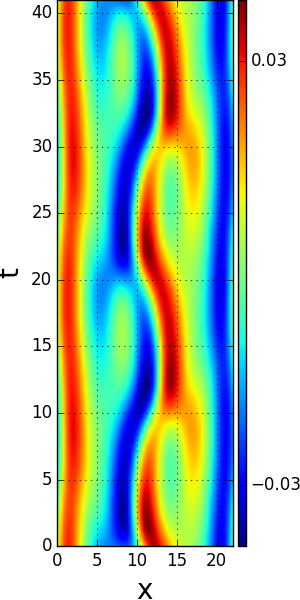
\includegraphics[width=\textwidth]{ppo1State64}
  \end{minipage}
  \begin{minipage}{.22\textwidth}
    \centering \small{\texttt{(b)}}
    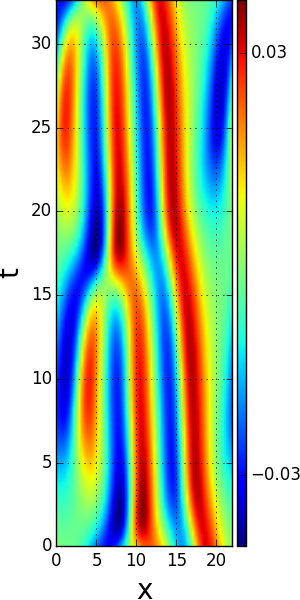
\includegraphics[width=\textwidth]{rpo1State64}
  \end{minipage}%
  \begin{minipage}{.55\textwidth}
    \centering \small{\texttt{(c)}}
    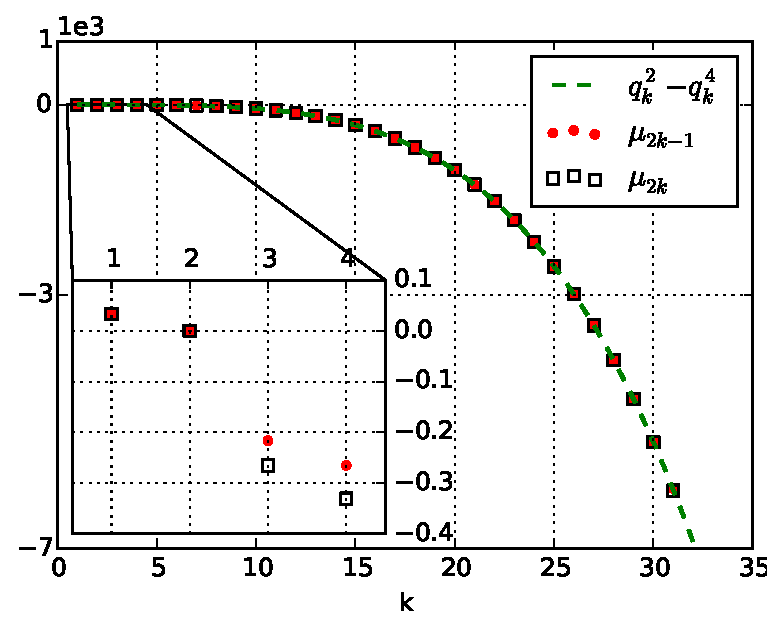
\includegraphics[width=\textwidth]{ppo1spectrum64}
  \end{minipage}
  \caption{(Color online)
    (a) Pre\po\ $\cycle{pp}_{10.25}$ and
    (b) \rpo\ $\cycle{rp}_{16.31}$ for total evolution time
    $4\,\period{pp}$ and $2\,\period{rp}$, respectively. The \edit{spatial} shift
    for $\cycle{rp}_{16.31}$ after one prime period $\simeq-2.863$.
    (c) The real parts of Floquet exponents paired for a given $k$ as
    $(k,\eigRe[2k-1])$ and $(k,\eigRe[2k])$, for $\cycle{pp}_{10.25}$ with
    truncation number $N=64$. The dashed line (green) is
    $q_{k}^{2}-q_{k}^{4}$. The inset is a magnification of the region
    containing the 8 leading \edit{exponents}.
  }
  \label{fig:ppo1rpo1}
\end{figure}
Our ultimate goal of implementing \ped\ is to analyze the stability
of periodic orbits and the associated stable/unstable manifolds in
dynamical systems, for the hope of getting a better understanding
of pattern formation and turbulence.
As an example, we focus on the one-dimensional \KSe\
\begin{equation}
u_t+\frac{1}{2}(u^2)_x+u_{xx}+u_{xxxx}=0\,,\; x\in [0,L]
\label{eq:ks}
\end{equation}
on a periodic spatial domain of size $L = 22$, large enough to exhibit
complex spatiotemporal chaotic dynamics\edit{\rf{SCD07}}.
This equation is formulated
independently by Kuramoto in the context of angular phase
turbulence in reaction-diffusion systems\rf{KurTsu75}, and
by Sivashinsky in the study of hydrodynamic instability in laminar
flames\rf{michsiv77}.
Periodic
boundary condition enables us to transform this partial differential
equation into a set of ODEs in Fourier space
\begin{equation}
\dot{a}_k \;\; =
( q_k^2 - q_k^4 )\, a_k
- i \frac{q_k}{2} \sum_{m=-\infty}^{\infty}a_m a_{k-m}
\label{eq:ksfourier}
\end{equation}
where $q_k = 2\pi k/L$, and the coefficients are complex,
$a_{k}=b_{k}+ic_{k}$. In our simulations, discrete Fourier transform
is used with $N=64$ modes ($k = -N/2 + 1$ up to $N/2$ in \eqref{eq:ksfourier}).

Since $u(x,t)$ is real, $a_{k}(t)=a^{*}_{-k}(t)$; thus, only half of the
Fourier modes are independent. As $\dot{a}_{0}=0$ from
\eqref{eq:ksfourier}, we can set $a_{0}=0$ corresponding to
zero mean velocity without loss of generality.
Also the nonlinear term
of $\dot{a}_{N/2}$ in fact has coefficient
\edit{$-i(q_{N/2} + q_{-N/2})/2 = 0$}
from symmetric consideration\rf{trefethenSpectral};
thus, $a_{N/2}$ is decoupled from other modes and it
can be set to zero as well. Thus, then the number of independent variables
is $N-2$,
\begin{equation}
\label{eq:fourierspace}
\hat{u}=(b_{1},c_{1},b_{2},c_{2},\cdots,b_{N/2-1},c_{N/2-1})^\top
\,.
\end{equation}
This is the `\statesp' in the discussion that follows. Exponential time-differencing
scheme combined with RK4\rf{cox02jcomp, ks05com}
is implemented to integrate
\eqref{eq:ksfourier}. The combination of \edit{\psd\ algorithm and reordering
algorithm is used to obtain all exponents and eigenvectors. In addition,
GEPP is stable for solving}
\eqref{eq:xdpsereal} and \eqref{eq:xdpsdcomplex} if the
time step in \KS\ integrator is not too \edit{large}.
\begin{table}[h]
  \footnotesize
  \centering
  \caption{
    The first 10 and last four \edit{Floquet multipliers
    $ \ExpaEig_i= \exp(\period{}\,\eigRe[i] \pm i\theta_{i})$ for
    orbits} $\cycle{pp}_{10.25}$ and $\cycle{rp}_{16.31}$, respectively.
    $\theta_{i}$ column lists either the phase,
    if the Floquet multiplier is complex, or `-1' if the
    multiplier is real, but inverse hyperbolic. Truncation number
    $N=64$.
  }
  \label{tab:floquet_ppo1}
  \begin{tabular}{l l c | l l c}
    \multicolumn{3}{c |}{$\cycle{pp}_{10.25}$} & \multicolumn{3}{c}{$\cycle{rp}_{16.31}$}\\
    $i$ & ~~~~~$\eigRe[i]$  & $\theta_{i}$  & $i$ & ~~~~~$\eigRe[i]$ & $\theta_{i}$  \\
    \hline
    1,2 & ~0.033209  &    $\pm$2.0079  &  1 &     ~0.32791  &              \\
    3 & -4.1096e-13  &                 &  2 &   ~2.8679e-12  &              \\
    4 & -3.3524e-14  &    -1           &  3 &   ~2.3559e-13  &              \\
    5 &  -0.21637    &                 &  4 &     -0.13214  &        -1    \\
    6,7 &  -0.26524  &   $\pm$2.6205   &  5,6 &   -0.28597  & $\pm$2.7724  \\
    8 &  -0.33073    &    -1           &  7 &     -0.32821  &       -1     \\
    9 &  -1.9605    &                  &  8 &      -0.36241  &             \\
    10 & -1.9676    &    -1            &  9,10 &   -1.9617  &  $\pm$2.2411 \\
    $\cdots$ &  $\cdots$    & $\cdots$ & $\cdots$ & $\cdots$ & $\cdots$   \\
    59 &  -5313.6   &    -1           &  59 &   -5314.4 &                 \\
    60 &  -5317.6   &                 &  60 &   -5317.7 &                 \\
    61 &  -6051.8   &    -1           &  61 &   -6059.2 &                 \\
    62 &  -6080.4   &                 &  62 &   -6072.9 &                 \\
    \hline
\end{tabular}
\end{table}

\KSe\ is equivariant under reflection and space translation: $-u(-x,t)$ and
$u(x+l,t)$ are also solutions if $u(x,t)$ is a solution, which corresponds
to equivariance of \eqref{eq:fourierspace} under group operation
 $R=\diag(-1,1,-1,1,\cdots)$ and $g(l)=\diag(r_{1},r_{2},\cdots,r_{N/2-1})$,
where
\[
r_{k}=
\begin{pmatrix}
  \cos(q_{k}l) & -\sin(q_{k}l) \\
  \sin(q_{k}l) & \cos(q_{k}l)
\end{pmatrix}
,\quad k=1,2,\cdots,N/2-1
\,.
\]
Based on the consideration of these symmetries,
there are three types of invariant orbits in \KS\ system: \po s in the
$b_k=0$ invariant antisymmetric subspace, pre\po s which are self-dual
under reflection, and \rpo s with a shift along group orbit after one
period. As shown in \refref{SCD07}, the first type is absent for a domain
as small as $L=22$, and thus we focus on the last two types of orbits.
For pre\po s $\hat{u}(0)=R\hat{u}(\period{p})$ , we only need to evolve
the system for a prime period $\period{p}$ which is half of the whole
period, with the Floquet matrix given by
$\jMps_{p}(\hat{u})=R\jMps^{\period{p}}(\hat{u})$. A \rpo,
$\hat{u}(0)=g_p\hat{u}(\period{p})$, returns after one period
$\period{p}$ to the initial state upon the group transform
$g_p=g(l_p)$, so the corresponding Floquet matrix is
$\jMps_p(\hat{u})=g_p\jMps^{\period{p}}(\hat{u})$. Here we show how {\ped} works
by applying it to one representative pre\po\ $\cycle{pp}_{10.25}$
and two
\rpo s $\cycle{rp}_{16.31}$ and $\cycle{rp}_{57.60}$
(subscript indicates the period of the orbit), described in
\refref{SCD07}.

\refFig{fig:ppo1rpo1} shows the time evolution of $\cycle{pp}_{10.25}$
and $\cycle{rp}_{16.31}$ and the Floquet spectrum of $\cycle{pp}_{10.25}$.
At each repeat of the prime period, $\cycle{pp}_{10.25}$ is invariant
under reflection along $x=L/2$, \reffig{fig:ppo1rpo1}\,(a), and
$\cycle{rp}_{16.31}$ has a \edit{fixed shift along the $x$ direction
after each period},
\reffig{fig:ppo1rpo1}\,(b). Since $\cycle{pp}_{10.25}$ and
$\cycle{rp}_{16.31}$ are both
time invariant and equivariant under SO(2) group transformation $g(l)$,
there should be two marginal Floquet exponents, corresponding to the
velocity field $v(x)$ and group tangent $t(x)=\mathbf{T}x$ respectively,
where $\mathbf{T}$ is the generator of SO(2) rotation:
\[
\mathbf{T}=\diag(t_{1},t_{2},\cdots,t_{N/2-1}),\quad
t_{k}=
\begin{pmatrix}
  0 & -q_{k} \\
  q_{k} & 0
\end{pmatrix}
\,.
\]
\refTab{tab:floquet_ppo1} shows that the $2_{nd}$ and $3_{rd}$,
respectively $3_{rd}$ and $4_{th}$ exponents of $\cycle{rp}_{16.31}$,
respectively $\cycle{pp}_{10.25}$, are marginal, with accuracy as low as
$10^{-12}$, to which the inaccuracy introduced by the error in the closure of
the orbit itself also contributes. \refTab{tab:floquet_ppo1} and
\reffig{fig:ppo1rpo1}\,(c) show that \psd\ is capable of resolving
Floquet multipliers differing by thousands of orders \edit{of magnitude}:
when $N=64$, the smallest Floquet multiplier \edit{magnitude }
for $\cycle{pp}_{10.25}$ is
$|\ExpaEig_{62}| \simeq e^{-6080.4\times 10.25}$.
\edit{This cannot be achieved if we try to compute a single
\JacobianM\ } for the whole orbit.
\refFig{fig:ppo1rpo1}\,(c) and \reftab{tab:floquet_ppo1} also
show that for \edit{large index} $k$, Floquet exponents almost lie on the
curve $(q_k^2 - q_k^4 )$. This is the consequence of
strong dissipation caused by the linear term in \eqref{eq:ksfourier} for
large Fourier mode index.
Also, Floquet exponents appear in pairs for large indices simply because
the real and complex part of high Fourier modes have a similar contraction
rate from \eqref{eq:ksfourier}.

\begin{figure}[h]
  \centering
  \begin{minipage}{.115\textwidth}
    \centering \small{\texttt{(a)}}
    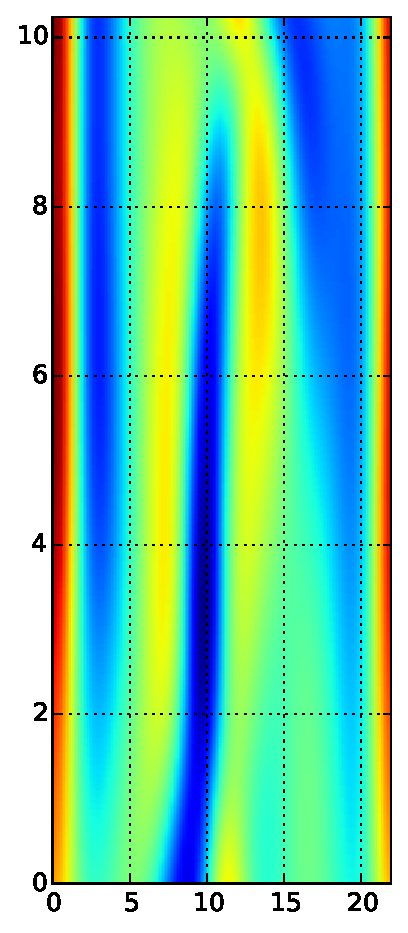
\includegraphics[width=\textwidth]{ppo1Fv1_64}
  \end{minipage}
  \begin{minipage}{.115\textwidth}
    \centering \small{\texttt{(b)}}
    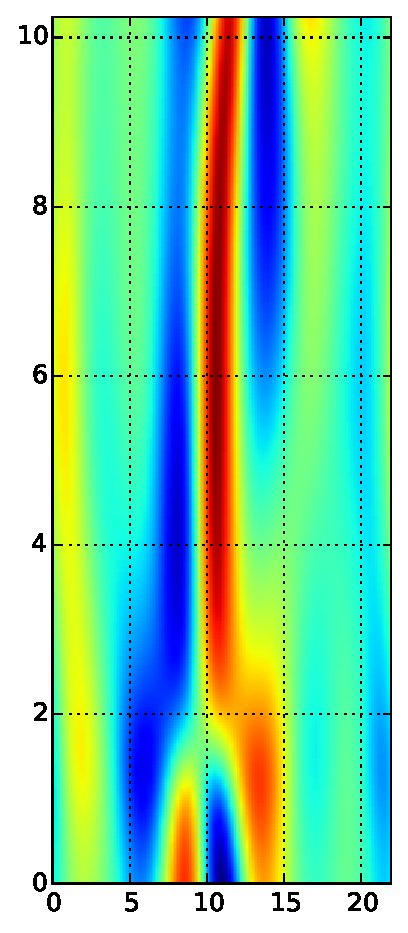
\includegraphics[width=\textwidth]{ppo1Fv5_64}
  \end{minipage}
  \begin{minipage}{.115\textwidth}
    \centering \small{\texttt{(c)}}
    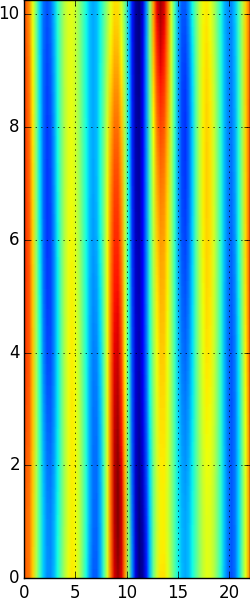
\includegraphics[width=\textwidth]{ppo1Fv10_64}
  \end{minipage}
  \begin{minipage}{.115\textwidth}
    \centering \small{\texttt{(d)}}
    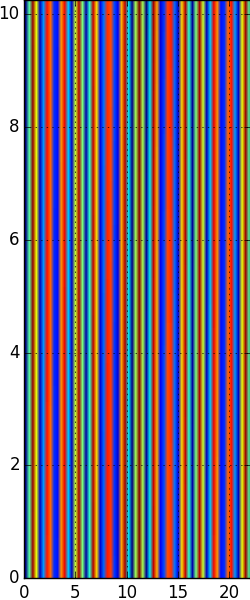
\includegraphics[width=\textwidth]{ppo1Fv30_64}
  \end{minipage}
  \begin{minipage}{.115\textwidth}
    \centering \small{\texttt{(e)}}
    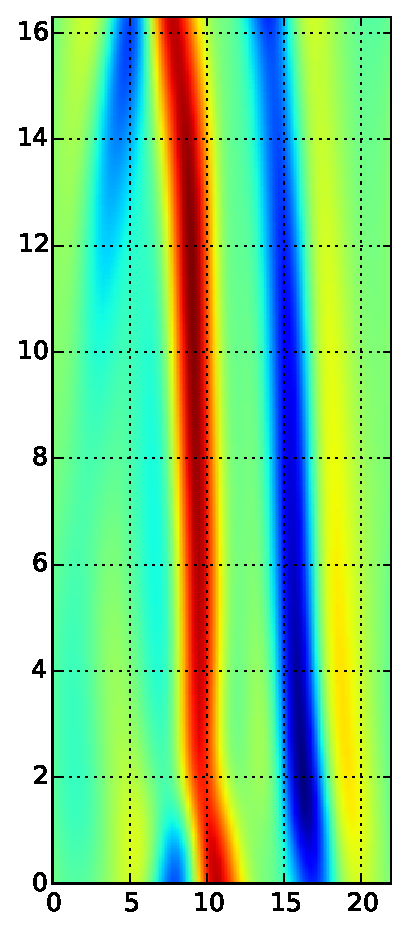
\includegraphics[width=\textwidth]{rpo1Fv1_64}
  \end{minipage}
  \begin{minipage}{.115\textwidth}
    \centering \small{\texttt{(f)}}
    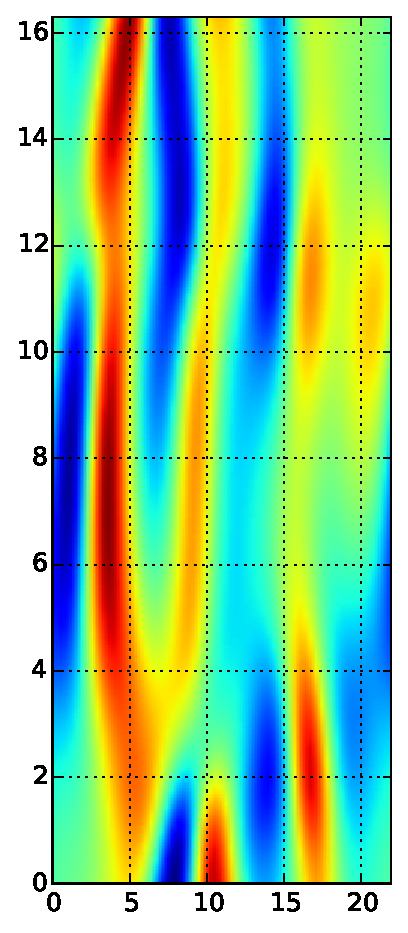
\includegraphics[width=\textwidth]{rpo1Fv4_64}
  \end{minipage}
  \begin{minipage}{.115\textwidth}
    \centering \small{\texttt{(g)}}
    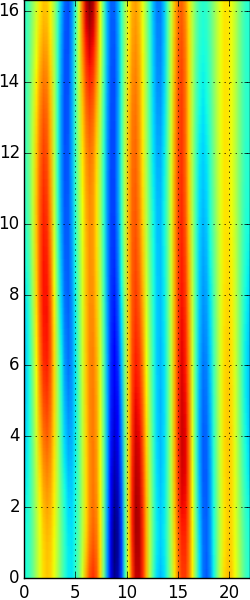
\includegraphics[width=\textwidth]{rpo1Fv10_64}
  \end{minipage}
  \begin{minipage}{.115\textwidth}
    \centering \small{\texttt{(h)}}
    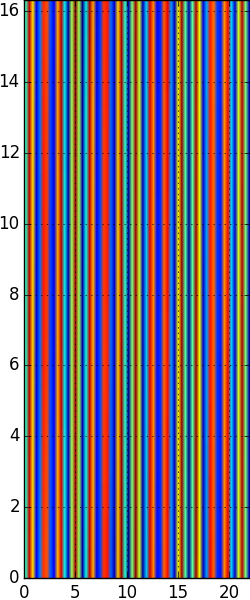
\includegraphics[width=\textwidth]{rpo1Fv30_64}
  \end{minipage}%
  \caption{(Color online)
    (a) $\sim$ (d) : the 1st (real part), 5th, 10th and 30th \Fv\ along
    $\cycle{pp}_{10.25}$ for one prime period.
    (e) $\sim$ (h) : the 1st, 4th (real part), 10th (imaginary part) 30th (imaginary part)
    \Fv\ along $\cycle{rp}_{16.31}$ for one prime period.
    Axes and color scale are the same as \reffig{fig:ppo1rpo1}.
  }
  \label{fig:Fvs}
\end{figure}
\begin{figure}[h]
  \centering
  \begin{minipage}{.47\textwidth}
    \centering \small{\texttt{(a)}}
    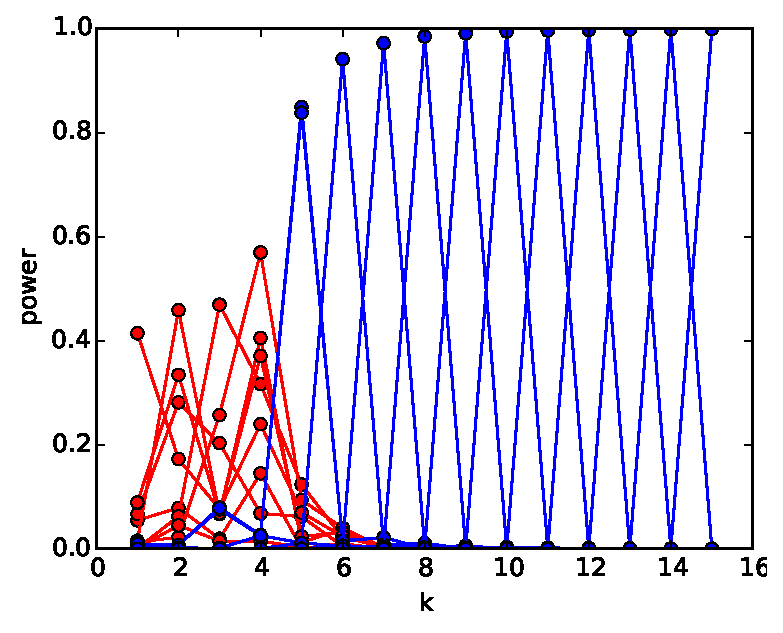
\includegraphics[width=\textwidth]{ppo1power64}
  \end{minipage}
  \begin{minipage}{.47\textwidth}
    \centering \small{\texttt{(b)}}
    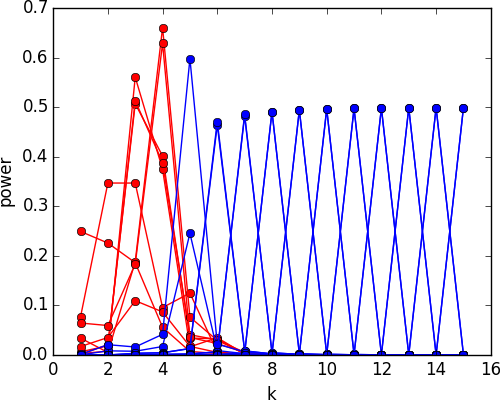
\includegraphics[width=\textwidth]{rpo1power64}
  \end{minipage}
  \caption{(Color online)
    The power spectrum of the first 30 \Fv s for $\cycle{pp}_{10.25}$
    (left) and $\cycle{rp}_{16.31}$ (right)
    at $\zeit=0$. Red lines correspond to the leading 8 \Fv s; while
    the blue lines correspond to the left 22 \Fv s with the $i_{th}$ one
    \edit{localized at index $\lceil \frac{i}{2} \rceil$.
    Power at index $k$ is defined to be the square of the $k_{th}$
    Fourier coefficient's magnitude
    of \Fv s}.
    The $x$-axis is
    labeled by the Fourier mode indices.
    Only the $k>0$ part is shown, and the part for
    negative $k$ follows by reflection. For complex \Fv s, the
    power spectra of the real part and imaginary part are calculated
    separately. Since almost all contracting \Fv s of $\cycle{rp}_{16.31}$
    form complex conjugate pairs, their power peaks are far less than 1,
    \edit{as shown in panel (b)}.
  }
  \label{fig:FVpower}
\end{figure}
\refFig{fig:Fvs} shows a few selected \Fv s along $\cycle{pp}_{10.25}$
and $\cycle{rp}_{16.31}$ for one prime period respectively. We need to
remind the reader that \Fv s for a whole period is obtained by solving
\eqref{eq:xdpsereal} or \eqref{eq:xdpsdcomplex}, not by evolving
\Fv s at one time spot to the later time spots because the evolution
procedure is not stable  for \Fv s. We can see that the leading
few \Fv s have turbulent structures containing only long waves
for both $\cycle{pp}_{10.25}$ and $\cycle{rp}_{16.31}$, but for
\Fv s corresponding to strong contraction rates, the configurations
are pure sinusoidal curves. The power spectra in \refFig{fig:FVpower}
demonstrate this point too. The leading 8 \Fv s have large components in
the first 5 Fourier modes and the spectra are entangled with each other;
while the remaining \Fv s almost concentrate
on a single Fourier mode and are decoupled from each other;
more specifically, the $i_{th}$ \Fv\ with $i\ge 9$
peaks at the $\lceil \frac{i}{2} \rceil_{th}$\footnote{\edit{
Here, $\lceil x \rceil$ denotes the smallest integer no less than $x$. }}
mode in \reffig{fig:FVpower}.
Takeuchi \edit{\etal}\rf{TaGiCh11, YaTaGiChRa08} observe similar
features in \cLv s along ergodic
trajectories and by measuring the tangency between these two groups of
\cLv s, they reach a reasonable conclusion about the dimension of
inertial manifold of \KSe\ and \cGLe.
Therefore, we anticipate that by analyzing the tangency of \Fv s along
different \po s can also lead to the same conclusion, which is our
future research.

\begin{figure}[h]
  \centering
  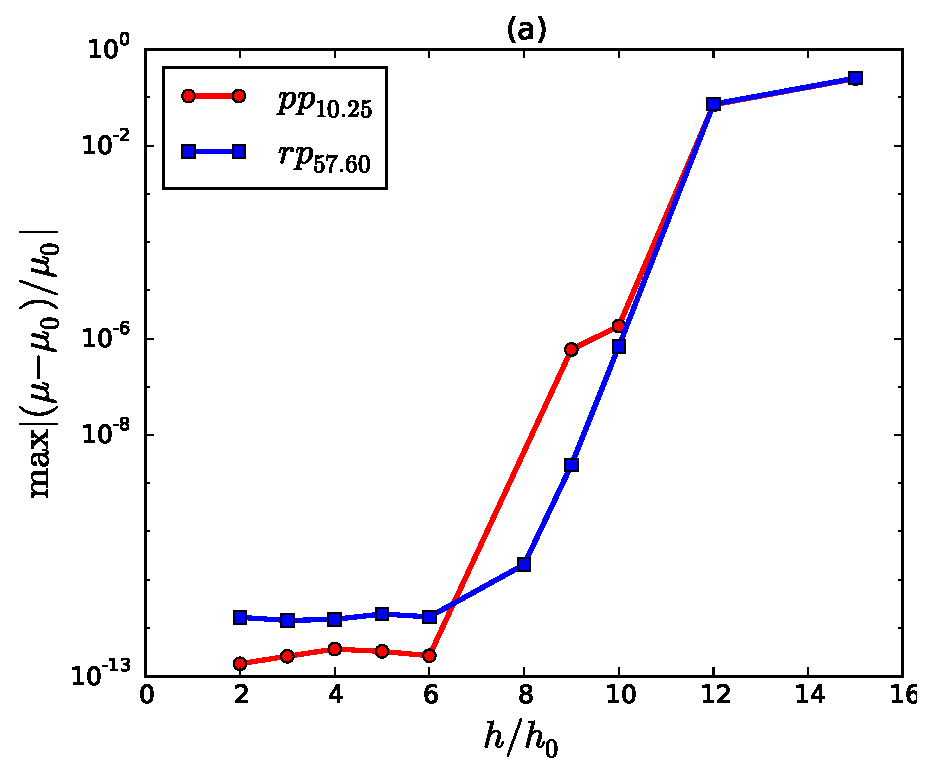
\includegraphics[width=0.47\linewidth]{ppo1FEerror} \hfill
  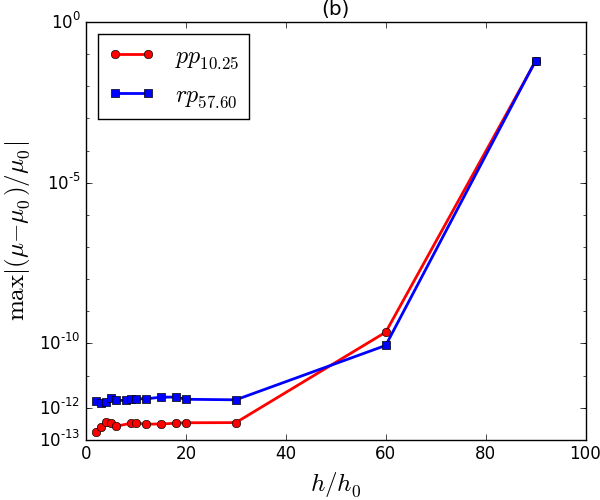
\includegraphics[width=0.47\linewidth]{rpo22FEerror}
  \caption{(Color online) Relative error of the real part of
    Floquet exponents associated with different time steps
    with which the Floquet matrix is integrated. Two orbits $\cycle{pp}_{10.25}$
    and $\cycle{rp}_{57.60}$ are used as an example with the base
    case $h_0 \approx 0.001$. (a) The maximal relative difference of
    the whole set of Floquet exponents with increasing time step (decreasing
    the number of ingredient segments of the orbit). (b) Only consider
    the first 35 Floquet exponents.}
  \label{fig:FEerror}
\end{figure}
\begin{figure}[h]
  \centering
  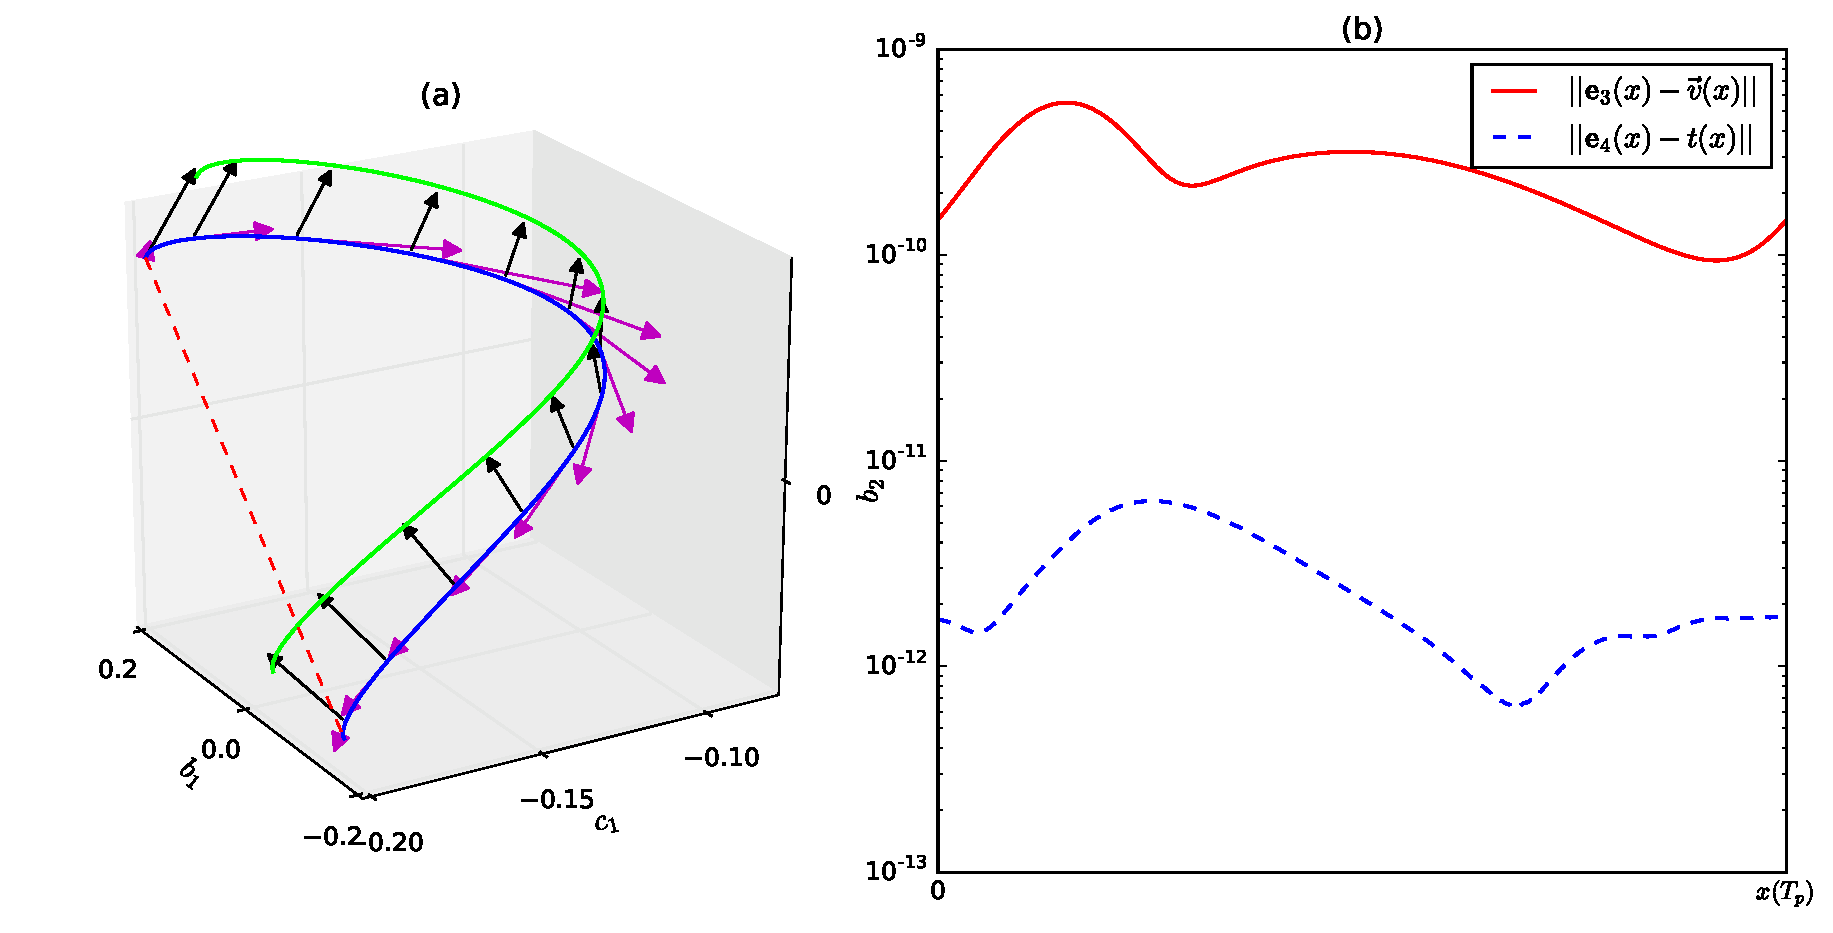
\includegraphics[width=1.0\linewidth]{ppo1vectfield}
  \caption{(Color online)
    Marginal vectors and the associated errors.
    (a) $\cycle{pp}_{10.25}$ in one period projected onto
    \edit{$[b_1, c_{1}, b_{2}]$}
    subspace (blue curve), and its counterpart (green line) generated by
    a small group transformation $g(\ell)$
    , here arbitrarily set to $\ell= \,L/(20\pi)$. Magenta and black
    arrows represent the first and the second marginal Floquet vectors
    $\jEigvec[3](x)$ and $\jEigvec[4](x)$ along the prime orbit.
    (b) The solid red curve is the \edit{Euclidean} difference between
    $\jEigvec[3](x)$ and the velocity field $\vec{v}(x)$ along the orbit,
    and the blue dashed curve is the difference between $\jEigvec[4](x)$ and
    the group tangent $t(x)=\mathbf{T}x$.
  }
  \label{fig:ppo1vectorfield}
\end{figure}
\begin{figure}[h]
  \centering
  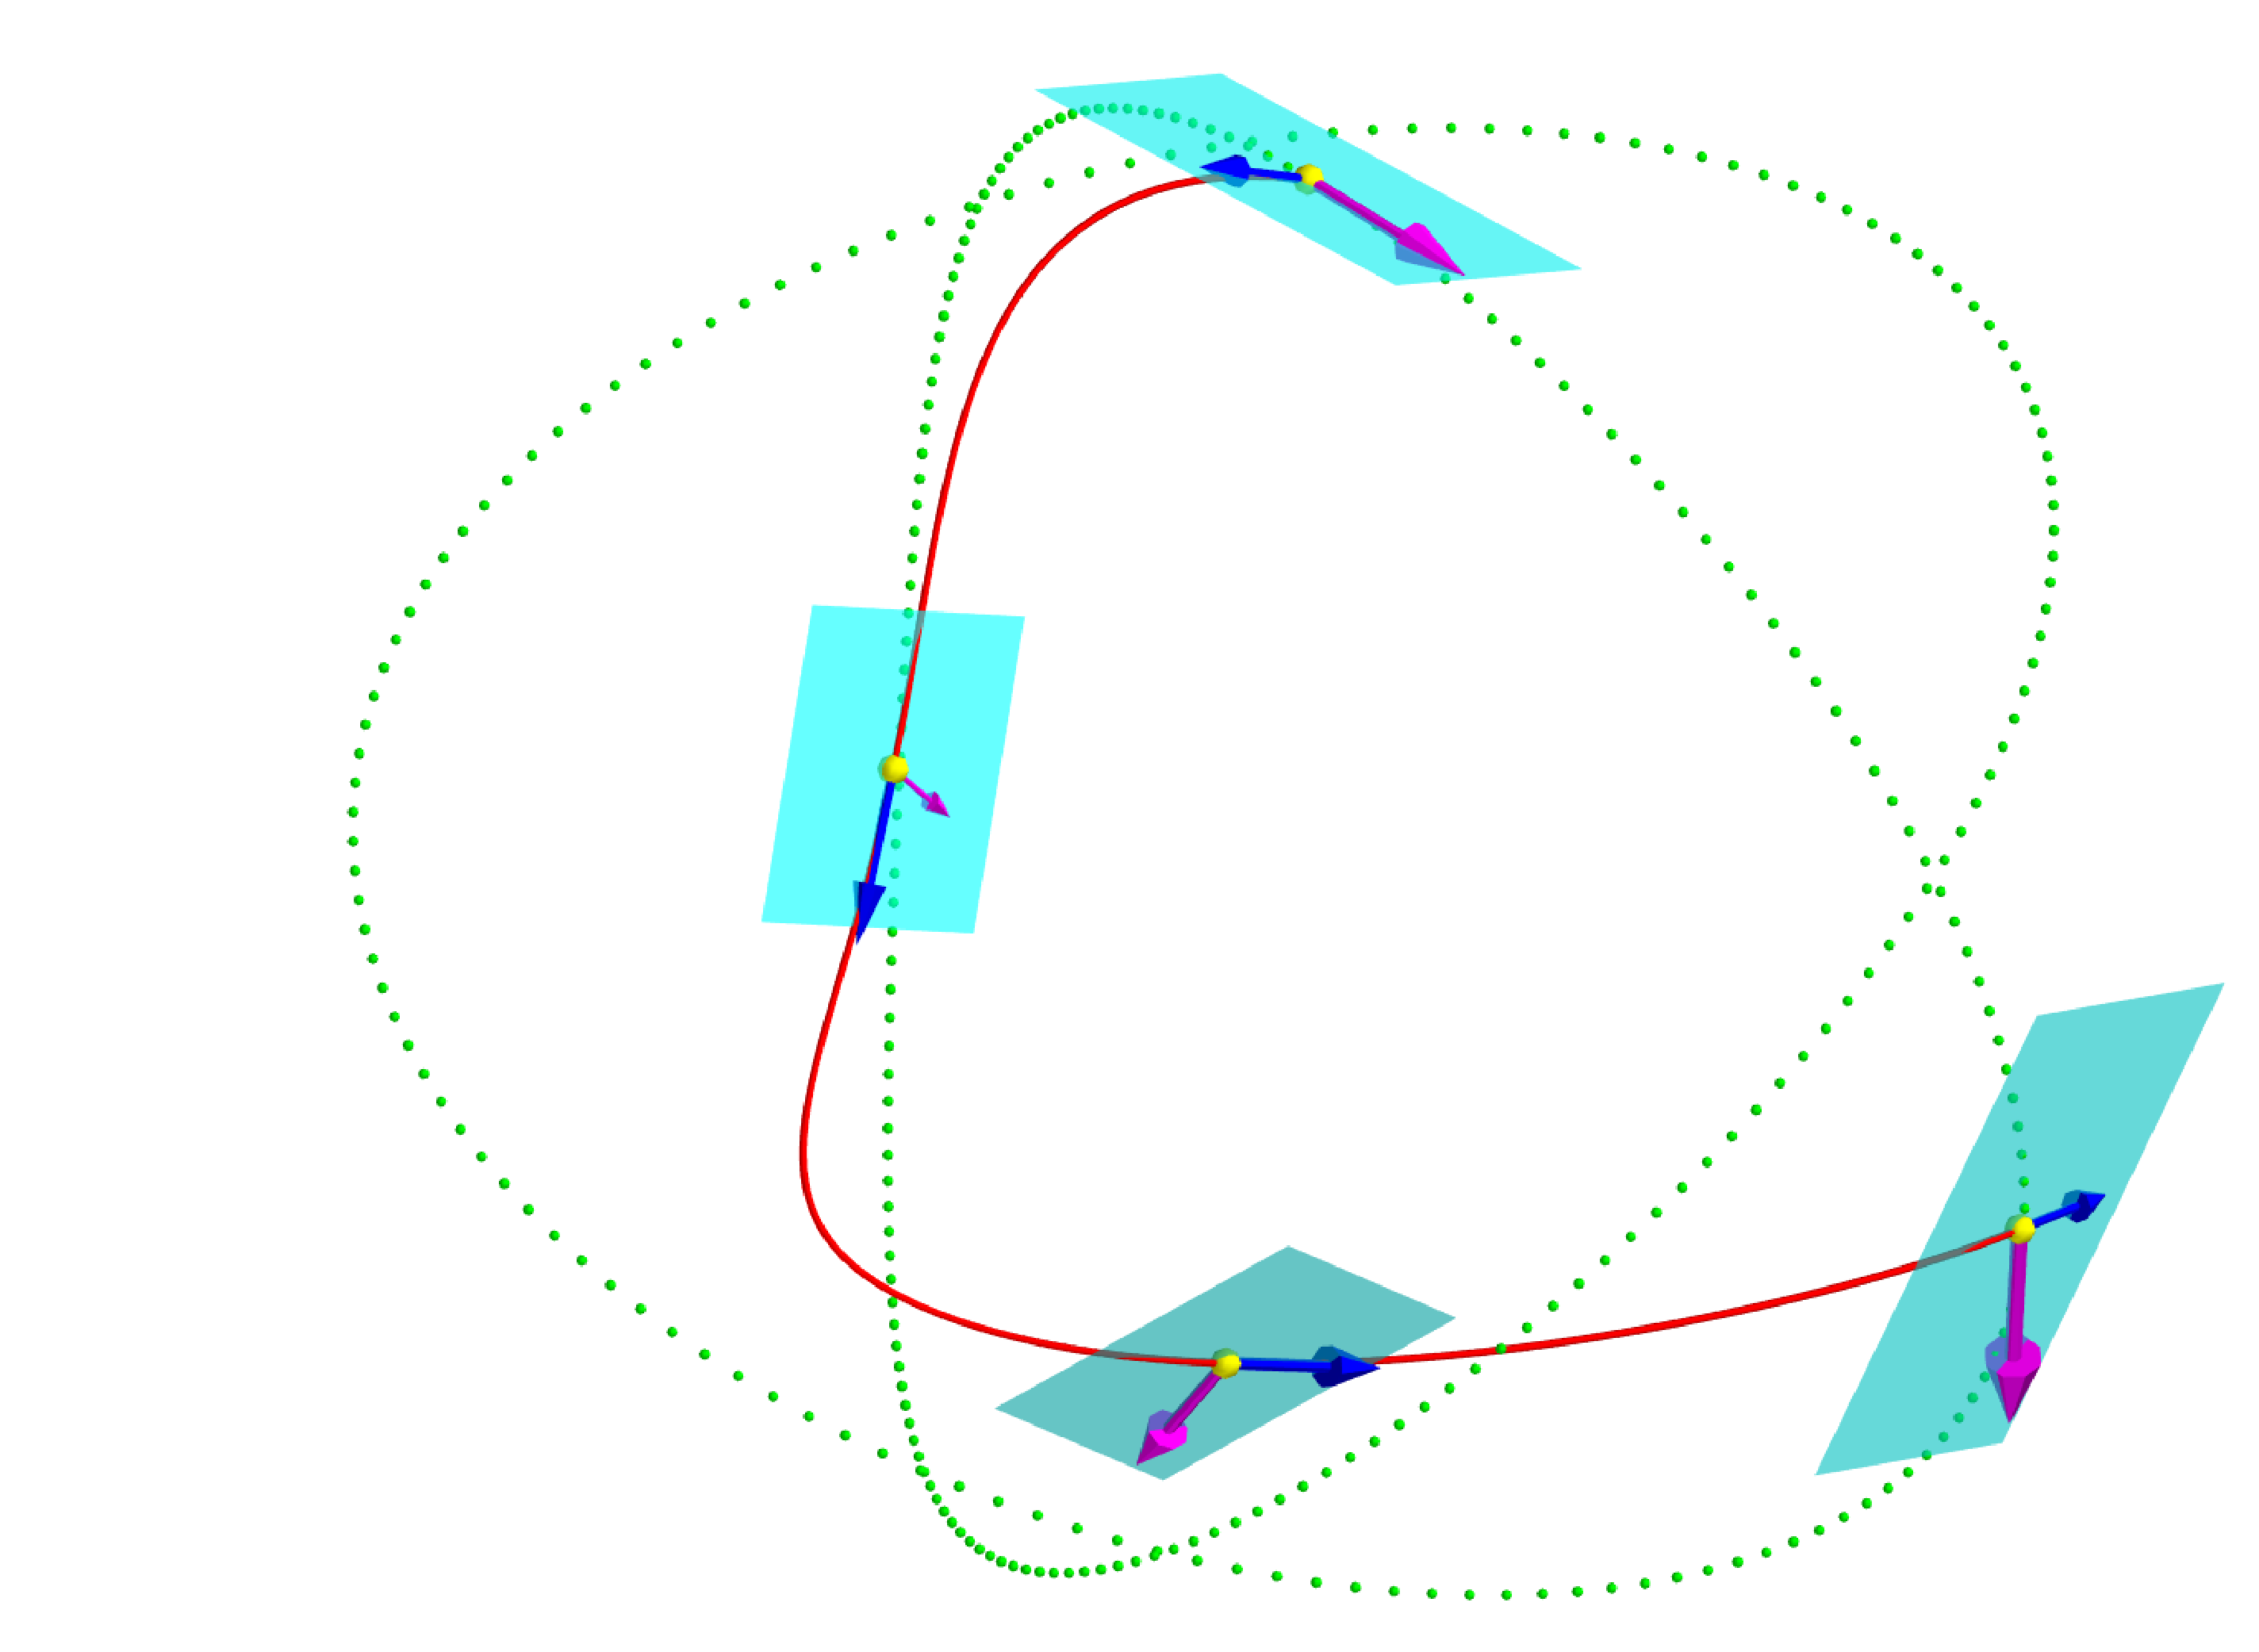
\includegraphics[width=0.7\linewidth]{rpo1_marginal3}
  \caption{
    (Color online) Projection of \rpo\ $\cycle{rp}_{16.31}$ onto
    the Fourier modes
    subspace $[b_2,c_2,b_3]$ (red curve). The dotted
     curve (lime) is the group orbit
    connecting the initial and final points. Blue and magenta arrows
    represent the velocity field and group tangent along the orbit,
    respectively. Two-dimensional planes (cyan) are spanned by the
    two marginal Floquet vectors at each point (yellow) along the orbit.
  }
  \label{fig:rpo1_marginal3}
\end{figure}

We have noted above that the \edit{semi-group property of \JacobianM}
\eqref{eq:xjacobian} enables us to factorize
$\ps{\jMps}{k}$ into a product of short-time matrices with matrix
elements of comparable \edit{order of magnitude}. In practice, caution should be
exercised when trying to determine the optimal number of time increments
that the orbit should be divided into. If the number of time increments
$m$ is too large, then, according to the estimates of
\refsect{sect:error}, the computation may be too costly. If $m$ is too
small, then the elements of \JacobianM\ corresponding to the
corresponding time increment may range over too many orders of magnitude,
causing \ped\ to fail to resolve the most contracting Floquet vector
along the orbit. One
might also vary the time step according to the velocity at a given point
on the orbit. Here we determined satisfactory $m$'s by numerical
experimentation shown in \reffig{fig:FEerror}. Since larger time step means
fewer time increments of the orbit, a very small time step ($h_0 \approx 0.001$)
is chosen as the base case, and it is increased to test whether the
corresponding Floquet exponents change substantially or not. As shown in
\reffig{fig:FEerror} (a), up to $6h_0$ the whole Floquet spectrum varies within
$10^{-12}$ for both $\cycle{pp}_{10.25}$ and $\cycle{rp}_{57.60}$. These
two orbits represent two different types of invariant solutions which have
short and long periods respectively,
so we presume that time step $6h_0$ is good enough
for other short or long orbits too. On the other hand, if only the first
few Floquet exponents are desired, the time step can be increased further
to fulfill the job. As shown in \reffig{fig:FEerror} (b), if we are only
interested in the first 35 Floquet exponents, then time step $30h_0$ is small
enough. In high dimensional nonlinear systems, often we are not interested in \edit{very contracting
directions because dynamics in these directions are transient} and shed little
insight into the system properties. Therefore, large time step could to used to
save time.


The two marginal directions have a simple geometrical interpretation and provide
a metric for us to measure the convergence of \ped.
\refFig{fig:ppo1vectorfield}\,(a) depicts the two marginal vectors of
$\cycle{pp}_{10.25}$ projected onto the subspace spanned
by \edit{$[b_1, c_{1}, b_{2}]$}
(the real, imaginary parts of the first mode and the real part of the
second Fourier mode). The first marginal \edit{direction} (the $3_{rd}$
Floquet vector in  \reftab{tab:floquet_ppo1}) is aligned with the velocity
field along the orbit, and the second marginal direction (the $4_{th}$
Floquet vector) is aligned with the group tangent. The numerical
difference between the unit vectors along these two marginal directions
and the corresponding physical directions is shown in
\reffig{fig:ppo1vectorfield}\,(b). The difference is under $10^{-9}$ and
$10^{-11}$ for these two directions, which demonstrates the accuracy of
the algorithm.
As shown in \reftab{tab:floquet_ppo1}, for a pre\po, such as $\cycle{pp}_{10.25}$,
the \edit{velocity field} and the group tangent have eigenvalue $+1$ and
$-1$ respectively, and are thus distinct. However, the two marginal
directions are degenerate for a \rpo, such as $\cycle{rp}_{16.31}$. So these two
directions are not fixed, but the
\edit{two dimensional plane spanned by them is uniquely
determined. \refFig{fig:rpo1_marginal3} shows that} the velocity field and
group tangent along orbit $\cycle{rp}_{16.31}$ indeed lie in the subspace spanned
by these two marginal directions.


\section{Conclusion and future work}
\label{sect:concl}

\edit{In this paper},
we use one-dimensional \KS\ system to illustrate the effectiveness
and potential wide usage of \ped\ applied to stability analysis
in dissipative nonlinear systems.
On the longer time scale, we hope to apply the method to
the study of orbits of much longer
periods, as well as to the study of high-dimensional, numerically exact
time-recurrent unstable solutions of the full Navier-Stokes equations.
Currently, up to 30 Floquet vectors for plane Couette invariant
solutions can be computed\rf{GHCW07}, but many more will be needed
and to a
higher accuracy in order to determine the physical dimension of a turbulent
Navier-Stokes flow. We are nowhere there yet; we anticipate the need for
optimizing and parallelizing such algorithms. Also, there is an opportunity
to apply \ped\ to Hamiltonian systems and we need additional tests to
show its ability to preserve symmetries of Floquet spectrum imposed by
Hamiltonian systems.


% \section{Acknowledgments}
\section*{Acknowledgments}

We are grateful to L.~Dieci for introducing us to complex
\psd, K.A.~Takeuchi for providing detailed documentation of his previous work
on \cLvs, R.L.~Davidchack for his database of periodic
orbits in \KSe, which is the basis of our numerical experiments,
and to
N.B.~Budanur,  E.~Siminos,  M.M.~Farazmand and H.~Chat\'e
for many spirited exchanges,
X.D. was supported by NSF grant DMS-1028133.
P.C. thanks
G.~Robinson,~Jr.\ for support.


%%%%%%%%%%%%%%%%%%%%%%%%%%%%%%%%%%%%%%%%%%%%%%%%%%%%%%%%%%%%%%%%%%%%
\bibliography{../bibtex/siminos}

%%%%%%%%%%%%%%%%%%%%%%%%%%%%%%%%%%%%%%%%%%%%%%%%%%%%%%%%%%%%%%%%%%%%
\ifboyscout
%\input ../lyapunov/DCTSCD14
\fi


\end{document}
